\documentclass[12pt]{article}

%\usepackage{src/cap/fontspec}
%\setmainfont{src/cap/Times New Roman}

\usepackage{tocbibind}

\usepackage[a4paper]{geometry}
\geometry{top=2.54cm, bottom=2.54cm, left=3.2cm, right=2.54cm}

\usepackage[spanish]{babel}
\usepackage[utf8]{inputenc}
\usepackage[T1]{fontenc}
\usepackage[none]{hyphenat}

\hyphenation{mi-cro-elec-tro-me-cá-ni-cos}
\hyphenation{ace-le-ró-me-tros}
\hyphenation{ca-pa-ci-ti-vos}

\usepackage{float}
\usepackage{graphicx} % graficos
\graphicspath{ {./images/} }
\usepackage{setspace}%interlineado agrega:
% \doublespacing \onehalfspace \singlespace \spacing{src/cap/x}
\spacing{1.5}
\setlength{\parindent}{0pt}
\pagestyle{headings}

%\usepackage {src/cap/ natbib }
\setlength{\parskip}{12pt}

\usepackage[backend=biber, autocite=inline, labeldateparts=true, maxcitenames=1,style = apa]{biblatex}

\addbibresource{bibliografias.bib}
\addbibresource{referencias.bib}

\usepackage{csquotes}
\usepackage[bookmarks = true, colorlinks=true, linkcolor = black, citecolor = black, menucolor = black, urlcolor = black]{hyperref}


\usepackage{enumitem}%eliminar el espaciado entre items de lista

\usepackage{array}%centrar verticalmente en tablas
%****************************************************
%     secciones con formato especifico
\usepackage{titlesec}
\titleformat{\section}[display]
{\normalfont\bfseries\LARGE}{\filcenter CAPÍTULO \thesection}{3pt}{\filcenter \LARGE}


\newcommand{\comillas}[1]{``#1"}

%  \makeatletter
%     \renewcommand{\l@section}[2]{\@dottedtocline{2}{1.6em}{1.6em}{#1}{}}
%  \makeatother


\begin{document}
\sloppy
\renewcommand{\listfigurename}{Índice de Figuras}
\renewcommand{\listtablename}{Índice de Tablas}
\renewcommand{\tablename}{Tabla}
\pagenumbering{roman}
	\setcounter{page}{0}
\begin{titlepage}

\begin{table}[t]
\centering
\begin{tabular}{ p{3cm} p{8.5cm} p{3cm} }
	\begin{flushleft}
\includegraphics[width=2.4cm]{logo_poli.png}\end{flushleft} &



	\begin{center}
	República Bolivariana de Venezuela\\
	Universidad Nacional Experimental Politécnica “Antonio José de Sucre”\\
	Vice Rectorado Barquisimeto \\
	Departamento de Ingeniería Electrónica\\

%***************************************************
%************** aqui va el titulo ******************
%***************************************************

	\vspace*{45mm}
	\begin{LARGE}Herramienta computacional para el análisis de la vibración en motores eléctricos alimentada mediante datos de una simulación digital\\\end{LARGE}

	\end{center}


	& \begin{flushright}
\includegraphics[width=1.7cm]{logo_electronica.jpg} \end{flushright}
\end{tabular}


	\vspace*{3mm}

	\parbox[c]{12cm}{

	}



    \vspace*{19mm}



\begin{flushright}
Integrantes:\\


Gerardo Alfonzo Campos Fonseca\\
V. 27085179\\
José Andrés Cortez Terán\\
V. 26540824\\

\vspace*{2mm}
Tutor: Dra. Luisa Mercedes Escalona\\
Cotutor: Dr. Carlos Zambrano\\

\end{flushright}
\vspace*{7mm}

\begin{center}Barquisimeto, Marzo 2022\end{center}
\end{table}
\end{titlepage}


    \thispagestyle{empty}

\begin{table}[t]
\centering
\begin{tabular}{ p{3cm} p{8.5cm} p{3cm} }
	\begin{flushleft}
\includegraphics[width=2.4cm]{logo_poli.png}\end{flushleft} &

	\begin{center}
	República Bolivariana de Venezuela\\
	Universidad Nacional Experimental Politécnica “Antonio José de Sucre”\\
	Vice Rectorado Barquisimeto \\
	Departamento de Ingeniería Electrónica\\

%***************************************************
%************** aqui va el titulo ******************
%***************************************************

	\vspace*{45mm}
	\begin{LARGE}Herramienta computacional para el análisis de la vibración en motores eléctricos alimentada mediante datos de una simulación digital\\\end{LARGE}

	\end{center}

	& \begin{flushright}
\includegraphics[width=1.7cm]{logo_electronica.jpg} \end{flushright}
\end{tabular}

    \vspace*{15mm}

\begin{flushright}
Integrantes:\\


Gerardo Alfonzo Campos Fonseca\\
V. 27085179\\
José Andrés Cortez Terán\\
V. 26540824\\

\vspace*{2mm}
Tutor: Dra. Luisa Mercedes Escalona\\
Cotutor: Dr. Carlos Zambrano\\

\end{flushright}

\vspace*{3mm}

\parbox[c]{12cm}{
    \begin{center}
        \begin{small}
            ``Trabajo Especial presentado ante el Departamento de Ingeniería
            Electrónica de la Universidad Nacional Experimental Politécnica
            ``Antonio José de Sucre"\ Vicerrectorado  Barquisimeto como requisito
            parcial para optar al título de Ingeniero Electrónico"

        \end{small}
    \end{center}
}

\vspace*{3mm}

\begin{center}Barquisimeto, Marzo  2022\end{center}
\end{table}


    \newpage
    \newpage
    
\thispagestyle{empty}
%\setcounter{figure}{0}
\phantom{}
\vfill
\begin{center}
   \it A nuestras familias y amigos por siempre estar presentes.
\end{center}
\vfill
\phantom{}


    
\addcontentsline{toc}{section}{AGRADECIMIENTOS}
%\setcounter{figure}{0}
\phantom{}
\vfill
\begin{center}
    Agradecemos primeramente a dios por darnos la vida y la  fuerza en los momentos
    más difíciles; a nuestros padres por criarnos, educarnos y siempre apoyarnos en
    nuestras metas; a nuestras familias por todo el amor, cariño y por ayudarnos y
    guiarnos en nuestra formación personal; a todas aquellas personas que ya no
    están con nosotros pero su recuerdo sigue en nuestras mentes y corazones; a
    nuestros amigos por darnos incontables buenos momentos y el escape de la rutina
    que muchas veces es necesario; a nuestros compañeros por su gran amistad, su
    apoyo incondicional y por ser personas que nos impulsan cada día a ser mejores
    en nuestra carrera; a nuestros profesores, sobre todo a los profesores del
    departamento de ingeniería electrónica por su gran vocación, su impecable ética
    de trabajo y su grandes conocimientos que no solo nos impulsan como
    profesionales sino también como  personas; a todo el personal universitario por
    su increíble labor en estos tiempos difíciles y finalmente pero no menos
    importante a nuestra universidad por brindarnos la oportunidad de demostrar
    nuestros conocimientos, de crecer y de formar parte de esta gran familia que
    siempre será parte de nuestros corazones.
\end{center}
\vfill
\phantom{}

	%\newpage
	\tableofcontents
	\newpage
	\listoffigures
	\newpage
	\listoftables

\spacing{1.2}
\thispagestyle{empty}
\addcontentsline{toc}{section}{RESUMEN}

    \begin{table}[t]
        \centering
        \begin{tabular}{ p{3cm} p{8.5cm} p{3cm} }
            \begin{flushleft}
\includegraphics[width=2.4cm]{logo_poli.png}\end{flushleft} &

                \begin{center}
                    República Bolivariana de Venezuela\\
                    Universidad Nacional Experimental Politécnica “Antonio José de Sucre”\\
                    Vice Rectorado Barquisimeto \\
                    Departamento de Ingeniería Electrónica\\

                \end{center}

                & \begin{flushright}
\includegraphics[width=1.7cm]{logo_electronica.jpg} \end{flushright}
        \end{tabular}


        \vspace*{0.6cm}

\parbox[c]{15cm}{
    \begin{center}
        \textbf{\large Herramienta computacional para el análisis de la vibración en
        motores eléctricos alimentada mediante datos de una simulación
        digital\\}


        \vspace*{1cm}
        \textbf{Autores:}\\
        Gerardo Alfonzo Campos Fonseca\\
        José Andrés Cortez Terán\\

        \textbf{Tutor:} Dra. Luisa Mercedes Escalona,
        \textbf{Cotutor:} Dr. Carlos Zambrano\\
    \end{center}
}
    \end{table}

        \section*{RESUMEN}

La presente investigación ha tenido como propósito el desarrollo de una
herramienta computacional para el análisis de la vibración en motores
eléctricos, haciendo uso de  datos obtenidos mediante una simulación
digital y una metodología de desarrollo
Web, enfocada a microservicios. Para lograrlo se desarrolló un modelo
estadístico, capaz de entregar las mediciones necesarias, a partir de una base
de datos real. Se
crearon 3 microservicios para la obtención, almacenamiento
(database as a service, DBaaS) y muestreo  de la información;
se desarrollaron estructuras de datos y una base de
datos no relacional para el almacenamiento de la información, se automatizó
la interconexión entre el modelo estadístico, el servidor de adquisición de
información y el DBaaS, mediante un cliente, y se despliega todo
el servicio en una página Web con 3 vistas, general, específica y
exhaustiva, que permiten observar una vista global del estado de
los motores, un recuento de la evolución histórica del
motor   y una gráfica  del espectro de
vibración que este posee;
además, la página consta de un  manual de usuario.
Se tiene un sistema  modular
 escalable en el tiempo que puede ser alimentado por cualquier sistema de
adquisición de datos que respete los formatos y estructuras definidas.

Palabras claves: servidor, microservicio, modelo estadístico, vibración,
motores eléctricos.


\spacing{1.5}
%***************************************************
%**********  Capitulo 1  ***************************
%***************************************************

\begin{refsegment}
	\newpage
    \begingroup
    \let\clearpage\relax
	\thispagestyle{empty}
\pagenumbering{arabic}
\setcounter{page}{5}

\section{PLANTEAMIENTO DEL PROBLEMA}

\subsection{DESCRIPCIÓN DEL PROBLEMA}

En la actualidad se vive un crecimiento exponencial a nivel industrial en todos
los rublos, desde manufactura hasta desarrollo de ciencias aplicadas,  especialmente
existe una muy alta demanda de alimentos, la evolución y la posibilidad de
satisfacer tal demanda es debido, entre
otras cosas, al motor eléctrico, este es un artefacto que transforma la
energía eléctrica en energía mecánica (movimiento), de manera que puede
impulsar el funcionamiento de una máquina y son utilizados ampliamente en:
Bombas para Agua, Bombas Industriales, Mezcladoras, Molinos, Correas
Transportadoras, Zarandas, Cortadoras, Ventiladores, Grúas, y en todo proceso
que involucre movimiento.

Adicional a la versatilidad de uso de los motores, existen factores que deben ser
considerados al evaluar su rendimiento, como las grandes pérdidas
(horas, insumos, dinero, etc.) que ocasiona una parada
de emergencia en una planta, por lo cual se considera de vital importancia que
los motores se encuentren completamente operativos y funcionales. Para
procurar su buen estado y funcionamiento, se deben realizar mantenimientos.

Existen diferentes tipos de mantenimiento, entre ellos están:
\begin{itemize}

\item{Correctivo: se espera que ocurra una falla para reparar o cambiar un
    equipo. Esto puede degradar la vida útil del equipo y debido a que la falla
        puede ocurrir en cualquier momento, lo que usualmente produce un paro en la
        línea de producción; por lo tanto, este tipo de mantenimiento suele y
        debe ser evitado.}

\item{Preventivo: para evitar una falla mayor se detiene la maquinaria para
    hacer un mantenimiento preparado con anticipación, se inspecciona la
        maquinaria y se reemplazan las piezas propensas a dañarse. Este tipo de
        mantenimiento en algunas circunstancias es más que suficiente pero en
        el caso de los rodamientos puede ser contraproducente.}

\item{Predictivo: se pronostica cuando una falla está a punto de ocurrir; a
    través de mediciones, y del estudio de las mismas, se prevé cuando un
        desperfecto está a punto de ocurrir y de esta forma se realiza una
        mejor planificación. Cabe resaltar que este tipo de mantenimiento puede
        dar información acerca del origen y la gravedad de las averías.}

\end{itemize}

En el caso de los motores eléctricos, como dice ~\textcite{Lacey}, el
mantenimiento preventivo tiene muchas desventajas dado que existen problemas de
índole mecánico así como administrativos y monetarios, un ejemplo de esto
pueden ser los altos costos de reemplazo dado que las partes se reemplazan muy
pronto, el riesgo de pérdida completa o parcial dado un error humano, como la posibilidad
de generar daño o una incorrecta instalación de la misma, la instalación de una
pieza defectuosa, y por último, el hecho de que las piezas reemplazadas
pueden tener muchos años de vida útil.

De esta forma se ve que una observación constante ofrece más control sobre las
variables mencionadas y, aunque no evita las posibilidades de error humano, si
permite reaccionar a este; adicionalmente, se deben considerar las altas
pérdidas y retrasos, sumadas a las dificultades administrativas, que generan
las paradas periódicas de la planta. Todas estas consideraciones son de suma
importancia ya que para poder ser ejecutadas se necesitan herramientas capaces de
dar a conocer el estado actual de una máquina y permitir a los operadores,
encargados o ingenieros tomar acciones cuando sean necesarias y de acuerdo a
las políticas de la empresa.

Por las razones expuestas surge la necesidad de reconocer las fallas y de tener
bajo continuo monitoreo los factores que las causan para, de esta forma,
atenuarlos. Según los estudios realizados por ~\textcite{Kammermann} la media
de la probabilidad de fallas en máquinas de inducción permanece al nivel de los
años 70 ($10^{-6}/hour$) y está altamente relacionada a la falla de los
rodamientos, y que un 59\% de las fallas son causadas por los rodamientos, esto
es debido a que son piezas sometidas a mucho estrés mecánico, permiten soporte
y asimismo necesitan tener poca fricción. Por esta razón, su principal falla es
el desgaste, de igual forma se presentan otras fallas estructurales que generan
vibraciones. Cabe resaltar que todas las fallas mecánicas generan vibración sin
importar su relación con los rodamientos y lo hacen a distinta frecuencia
($f$).

Por lo expuesto, es de suma importancia el estudio de la vibración, para la que
se suele implementar un acelerómetro y con un estudio de la frecuencia se puede
obtener la causa y la magnitud de la falla y de esta forma programar su
reparación. Sin embargo, debido a que esta evaluación debe ser realizada en
cada rodamiento y acople o extensión del motor  y dadas las mediciones que se
deben realizar por unidad (motor y acoples) y por la gran cantidad de unidades
existentes a nivel industrial, es virtualmente imposible el estudio con un
acelerómetro convencional (a pesar de que la medición no sea un proceso muy
largo y los cálculos y evaluaciones sean realizados posteriormente). Sumado a
esto, las industrias suelen poseer medidas y controles sanitarios, aumentados
por la pandemia actual, que no permiten el constante monitoreo de la planta
significando esto la imposibilidad de implementar este tipo de acciones de
forma manual, por lo cual se debe recurrir a un sistema de automatización capaz
de medir las vibraciones en todos estos equipos que, a su vez, permita el
estudio de estos datos de forma remota.

%	
%\subsection{solución}

%Para llevar a cabo lo expuesto anteriormente %en el planteamiento del problema
Para esto, se plantea la implementación de un sistema capaz de tomar datos de forma continua y enviarlos a un servidor el cual permita el almacenar, estudiar y muestrear la información en distintos niveles de profundidad, con respecto al análisis realizado.\\
Para esto se plantea una simulación digital, diagramada en la figura \ref{fig:diagrama}, que constara de un análisis estadístico para obtener las medidas típicas de un acelerómetro en motores eléctricos con distintos niveles de daños, esta data permitirá, después de ser almacenada en una base de datos y procesada, generar 3 niveles de análisis:\\
\begin{itemize}
\item La vista principal, permitirá observar una cantidad especifica de motores, simbolizando los existentes en una planta o piso, y su estado general.

\item La vista especifica, dará la información actual e histórica referente a un único motor previamente seleccionado.

\item La vista exhaustiva se refiere a un análisis en frecuencia de la vibración de un motor especificado con anterioridad, con la finalidad de permitir al operador o ingeniero encargado determinar la causa de las posibles averías.
\end{itemize}


Y finalmente, toda esta información y opciones se mostrarían a través de una pagina web para facilitar su acceso.

\begin{figure}[htb]
\centering
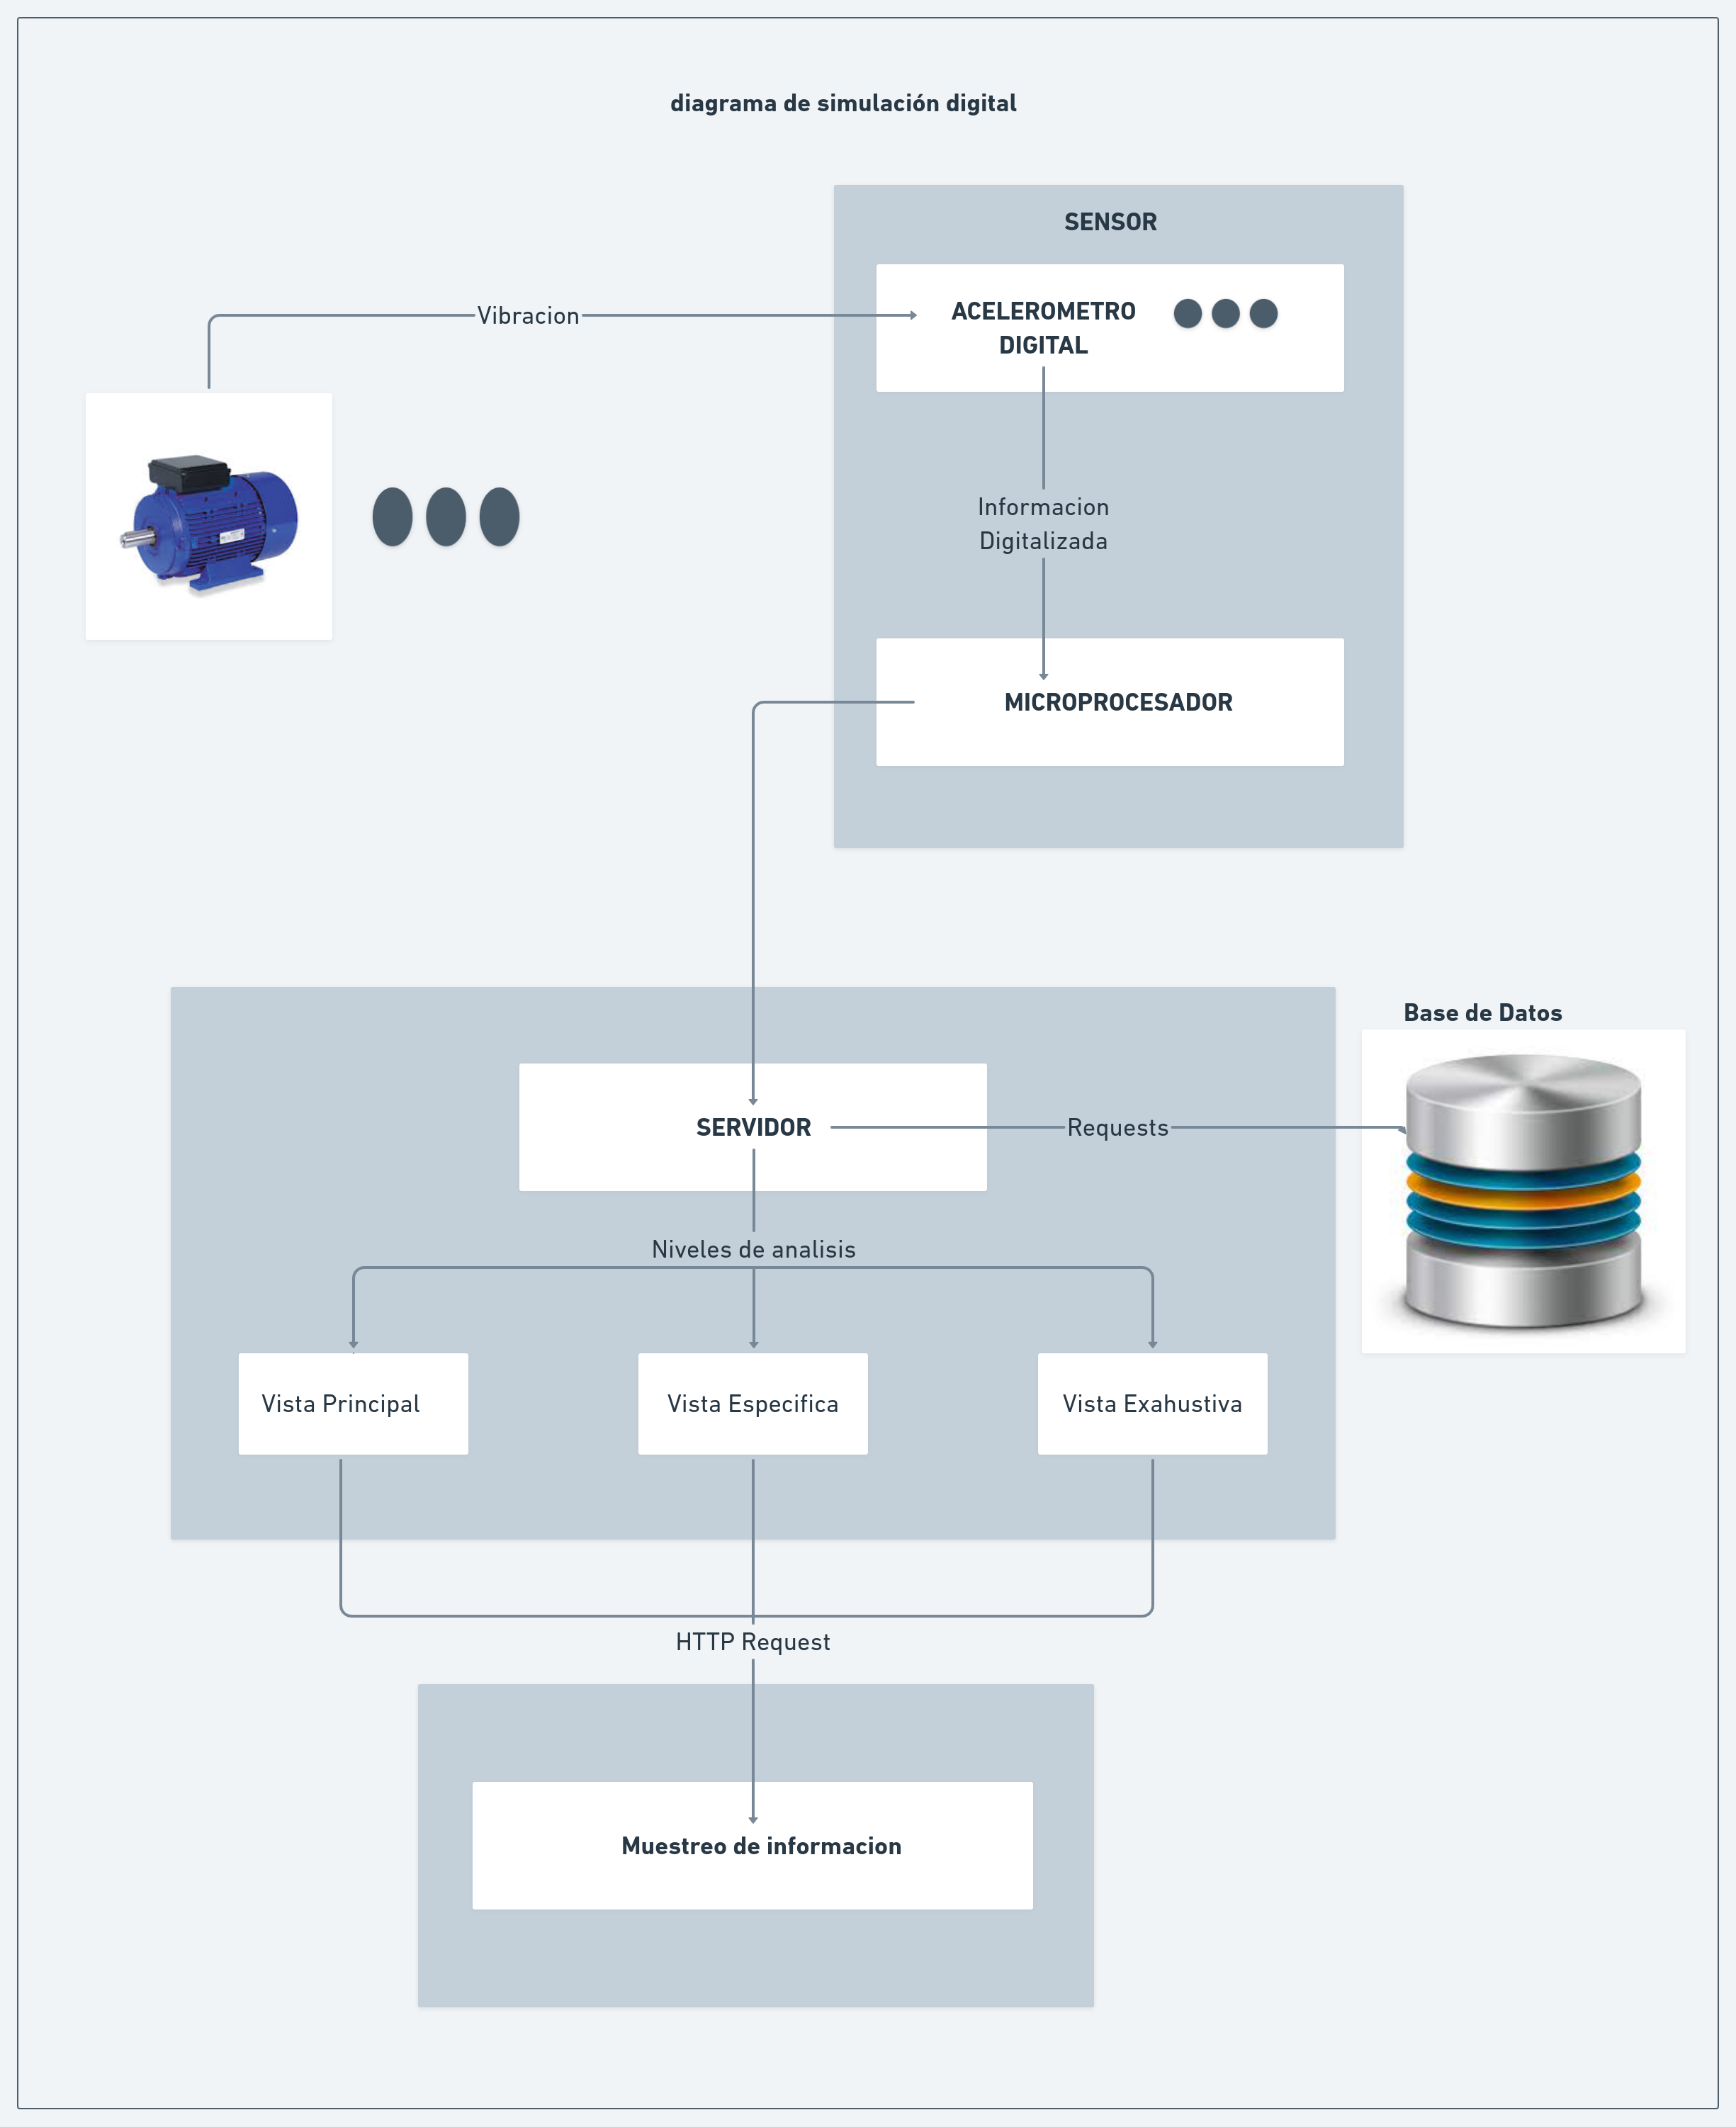
\includegraphics[width=15cm]{Diagrama_sensorica.png}
\caption{Diagrama de la simulación digital}
\label{fig:diagrama}
\end{figure}



	\subsection{OBJETIVOS DE LA INVESTIGACIÓN}

\subsubsection{Objetivo general}
	Desarrollar una herramienta computacional para el análisis de la vibración en motores eléctricos, mediante la simulación digital de un acelerómetro, con la finalidad de que un operador determine averías y sus causas.


\subsubsection{Objetivos específicos}

	\begin{enumerate}
		\item Justificar la escogencia de las herramientas y lenguajes a utilizar en las diferentes etapas que requiere la simulación. (José Cortez y Gerardo Campos)

		\item Generar un modelo estadístico de la vibración en motores eléctricos con distinto grado de daño utilizando una base de datos de la salida de un acelerómetro digital. (José Cortez)

		\item Elaborar una base de datos con información obtenida del modelo estadístico para alimentar los niveles de análisis de la herramienta. (José Cortez y Gerardo Campos)

		\item Realizar análisis de fallas en frecuencia, a partir de la salida del modelo del acelerómetro. (Gerardo Campos)

		\item Mostrar la información solicitada de acuerdo al nivel de análisis seleccionado. según sea: Vista Principal, Vista Específica o Vista Exhaustiva. (José Cortez y Gerardo Campos)

		\item Elaboración de una página Web para facilitar la utilización del sistema. (José Cortez y Gerardo Campos)

		\item Comprobar los resultados de la herramienta de análisis. (José Cortez y Gerardo Campos)
	\end{enumerate}

	\subsection{JUSTIFICACIÓN E IMPORTANCIA}

Para prevenir las fallas mecánicas que ocurren en los motores, por el deterioro
y desgaste de los rodamientos, estos se deben tener bajo constante monitoreo
para poder efectuar un mantenimiento puntual que elimine dichos peligros. De
esta forma el mantenimiento predictivo es la clave para mejorar la vida útil,
funcionamiento y planificación de todo proceso especialmente a niveles
industriales, donde la cantidad de motores eléctricos es bastante elevada
por lo cual la automatización del proceso es crucial.

Sin embargo, dado los altos costos que implican realizar una automatización y
en especial a escalas industriales se suele hacer una simulación o una
emulación para estudiar y obtener el modelo más preciso, gracias a la facilidad
de manipular con mayor eficacia los diseños y conocer su comportamiento real
sin necesidad de construirlo, antes de realizar la implementación y todo el
proceso que esta conlleva.

Habiendo expuesto la importancia del mantenimiento como también la de realizar
simulaciones, se justifica el hecho de realizar el desarrollo del trabajo aquí
propuesto el cual permita emular el comportamiento y las salidas de un
acelerómetro, como también otorgar las herramientas necesarias para
realizar un mantenimiento predictivo, y de esta forma estudiar a
profundidad su estado actual como también su evolución histórica. Todo esto
sumado a las facilidades de portabilidad que ofrece un sistema Web, facilitando
la revisión constante sin las dificultades de los protocolos de acceso y
sanidad usuales en las plantas industriales.

	
\subsection{LIMITACIONES Y ALCANCES}
    En función de los objetivos planteados con anterioridad, se puede definir
    tanto las limitaciones como el alcance del proyecto.

\subsubsection{Limitaciones}
\begin{itemize}
    \item Recursos económicos impiden la adquisición de dispositivos para
        pruebas en motores reales.

    \item Disponibilidad de muestras, aunque se cuenta con una base de datos lo
        suficiente grande para cubrir el comportamiento de la vibración en
        motores, incluso de distinta potencia, esta es discreta y con
        intervalos de tiempo considerables entre cada muestra.


    \item Las establecidas por el software de terceros utilizado en el diseño
        y desarrollo del proyecto.
\end{itemize}

\subsubsection{Alcance}
    El principal alcance de este trabajo es el desarrollo de una herramienta
    computacional para el análisis de la vibración en motores eléctricos; en
    función de esto:

	\begin{itemize}
        \item La herramienta computacional permite una vista general del estado
            de todos los motores en un espacio previamente delimitado y
            seleccionado (planta o piso) que se encuentren en la base de datos.

        \item La herramienta computacional permite una vista detallada del
            estado de un motor seleccionado, previamente por el usuario, que se
            encuentre en la base de datos.

        \item El sistema cuenta con una base de datos a partir de la cual se
            desarrollarán los resultados ofrecidos.

        \item No se contempla la construcción de hardware de ningún tipo.


	\end{itemize}

    \endgroup


%***************************************************
%**********  Capitulo 2  ***************************
%***************************************************
%
%\subsection{solución}

%Para llevar a cabo lo expuesto anteriormente %en el planteamiento del problema
Para esto, se plantea la implementación de un sistema capaz de tomar datos de forma continua y enviarlos a un servidor el cual permita el almacenar, estudiar y muestrear la información en distintos niveles de profundidad, con respecto al análisis realizado.\\
Para esto se plantea una simulación digital, diagramada en la figura \ref{fig:diagrama}, que constara de un análisis estadístico para obtener las medidas típicas de un acelerómetro en motores eléctricos con distintos niveles de daños, esta data permitirá, después de ser almacenada en una base de datos y procesada, generar 3 niveles de análisis:\\
\begin{itemize}
\item La vista principal, permitirá observar una cantidad especifica de motores, simbolizando los existentes en una planta o piso, y su estado general.

\item La vista especifica, dará la información actual e histórica referente a un único motor previamente seleccionado.

\item La vista exhaustiva se refiere a un análisis en frecuencia de la vibración de un motor especificado con anterioridad, con la finalidad de permitir al operador o ingeniero encargado determinar la causa de las posibles averías.
\end{itemize}


Y finalmente, toda esta información y opciones se mostrarían a través de una pagina web para facilitar su acceso.

\begin{figure}[htb]
\centering
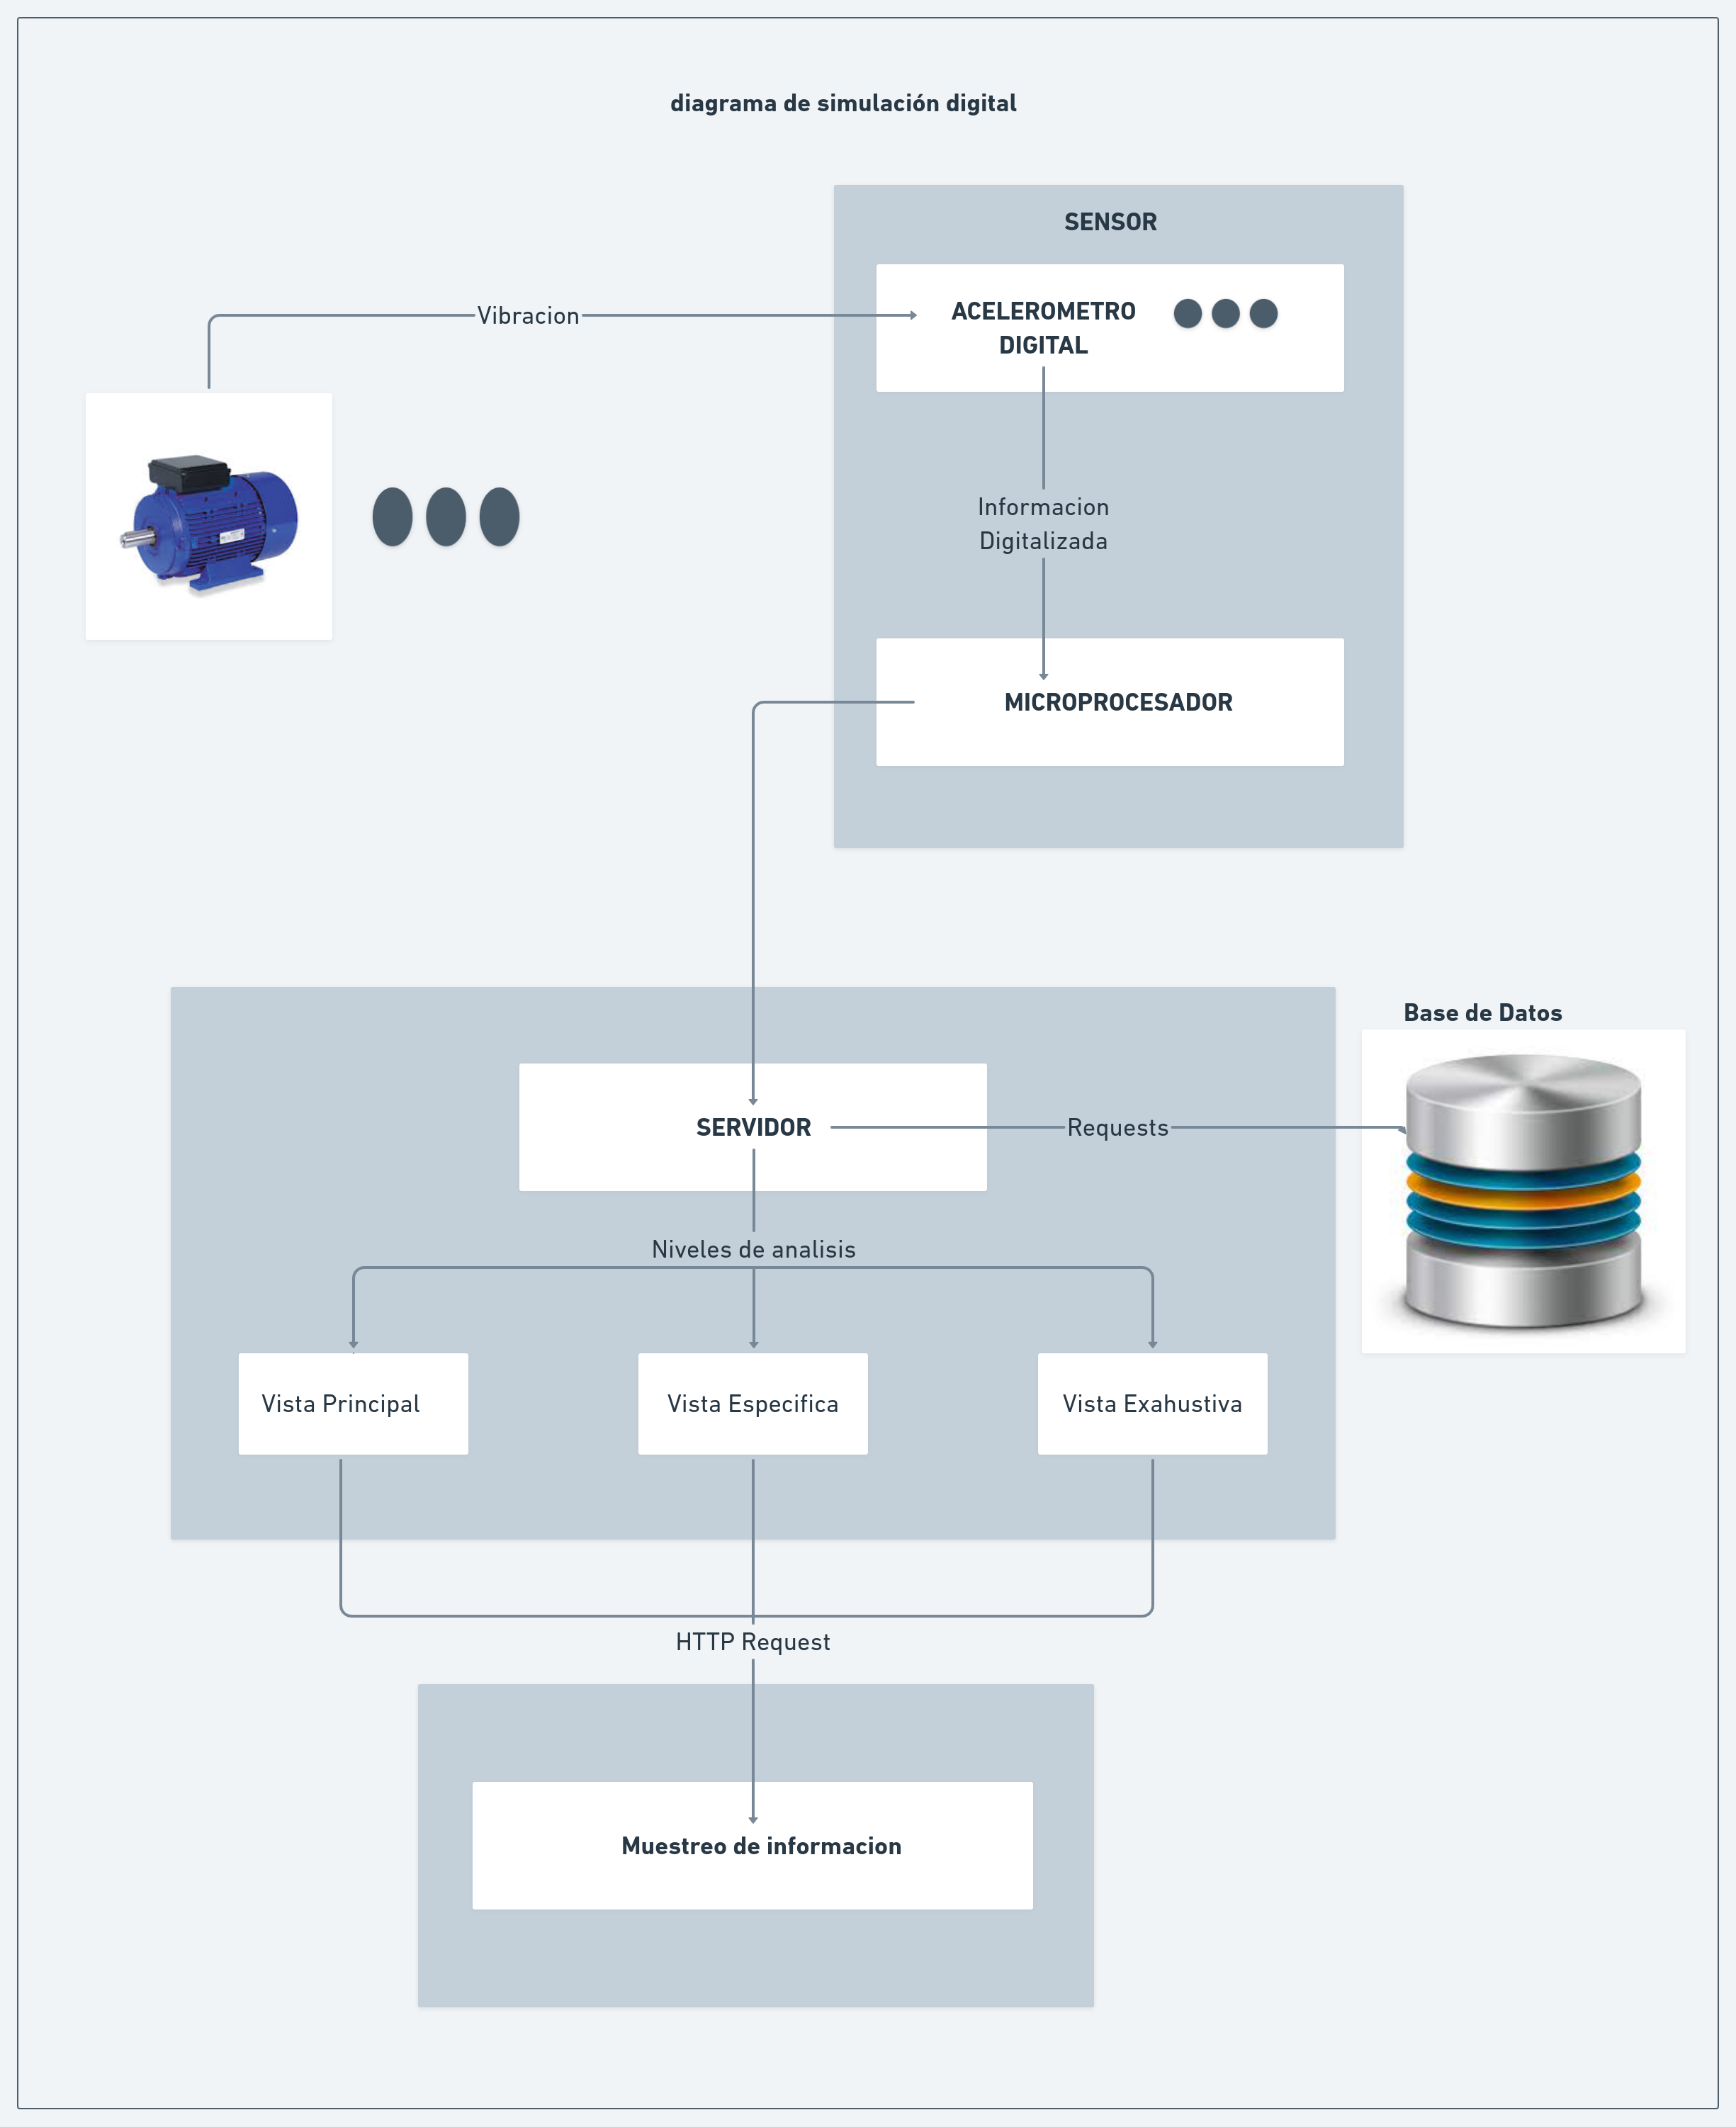
\includegraphics[width=15cm]{Diagrama_sensorica.png}
\caption{Diagrama de la simulación digital}
\label{fig:diagrama}
\end{figure}




	\newpage
    \begingroup
    \let\clearpage\relax
	\thispagestyle{empty}

\section{REVISIÓN BIBLIOGRÁFICA}

\subsection{ANTECEDENTES}

\textcite{Ramazan} Describen un modelo estadístico sobre el deterioro de
motores eléctricos de inducción. El artículo clasifica el deterioro del motor
en 7 etapas de acuerdo al nivel de vibración de sus rodamientos. Este
antecedente es de gran utilidad para realizar el modelo estadístico que alimenta
la base de datos ya que proporciona bases teóricas y un ejemplo práctico.

\textcite{Pinto} realizan una simulación de redes de sensores inalámbricos, con
el fin de mejorar la detección de fallas de los sensores. Esta simulación fue
realizada con Castalia un simulador de redes de sensores inalámbricos y el
sensor usado fue un detector de luminosidad. Algunas de las razones que
menciona el artículo de por qué fue escogida una simulación es debido a que
realizar el experimento con sensores requiere un costo elevado de hardware y un
estudio analítico no es efectivo, ya que la complejidad del sistema es muy
grande. Este trabajo es de utilidad debido a que sirve como orientación a la
elaboración de la simulación del sensor que generaría el modelo estadístico.

\textcite{Ugwiri} Presentan un resumen de las técnicas más usadas actualmente
en la detección de fallas en motores eléctricos mediante análisis de vibración,
además de realizar un experimento donde se ponen a prueba algunos de estos
conceptos. El propósito de este antecedente es el de apoyar la elaboración del
modo de "vista exhaustiva".

\textcite{Koene} Elaboran un sensor de vibración inalámbrico de código libre
llamado Memsio. Este dispositivo es alimentado por baterías y permite la
adquisición de datos a alta velocidad por medio del uso de un acelerómetro
microelectromecánico. Los autores mencionan que en la industria los sensores de
aceleración más usados son los piezoeléctricos, debido a tener una mayor
precisión y tolerancia al ruido, sin embargo, los avances de los dispositivos
microelectromecánico y su bajo costo hacen cada vez más factibles su uso para
el monitoreo. Este antecedente muestra la tendencia de la reducción de precios
de los sensores inalámbricos lo cual apoya al propósito del trabajo al hacer
factible las redes de sensores.

\textcite{Soto-Ocampo} Elaboraron un sensor de vibración multicanal para
vibraciones de alta frecuencia utilizando una Raspberry pi. El objetivo del
proyecto era conseguir una alternativa de bajo costo, para poder monitorizar
la salud de rodamientos en motores eléctricos, pero sin sacrificar la calidad de
la medición porque, como explican los autores del artículo, la mayoría de las
fallas en los rodamientos ocurre a altas frecuencias y muchas de las
alternativas de bajo costo no alcanzan la frecuencia necesaria. Este antecedente
es de utilidad dada la cantidad de información, tanto teórica como datos de
simulación, que provee.



	\subsection{MARCO TEÓRICO}

Esta parte del capítulo expone el contenido teórico necesario para la
realización de este proyecto. Esto incluye información sobre los motores
eléctricos,  análisis de la vibración, las herramientas computacionales, los
sistemas, y el modelado estadístico.

%https://es.wikipedia.org/wiki/Motor_el%C3%A9ctrico


\subsubsection{ Motores eléctricos}

De acuerdo a \Cite{Fraile}, un motor eléctrico es un dispositivo que
transforma energía eléctrica en
energía mecánica mediante la acción de campos magnéticos y están compuestos,
principalmente, por un estator (parte fija) y un rotor (parte móvil).
Existen dos familias principales de motores eléctricos las cuales, a su vez,
se subdividen en \textbf{motores de corriente alterna} como lo son los  motores
de inducción, síncronas, entre otros y los \textbf{motores de corriente continua}
como lo son los motores de escobillas,  sin escobillas, de imán permanente,
entre otros.

El motor más usado en el sector industrial, es el motor de inducción, debido
principalmente a su bajo costo y al poco mantenimiento que requiere para estar
completamente operativo, esto en particular es debido a su sencillo diseño
en comparación al de otros motores de igual potencia, ya que requiere  menor
número de componentes. Cabe resaltar que el segundo tipo de motor más usado es
el motor de corriente
continua, debido a que su control, en términos de torque y potencia, es mucho
mas sencillo para ciertos niveles de potencia.

También existen los motores síncronos, cuya construcción es similar a la de un
motor de inducción pero a su vez requiere de una fuente de alimentación externa
para el rotor, lo cual aumenta su costo, además de esto su velocidad es
constante, por lo tanto este tipo de motor es utilizado en aplicaciones
específicas. Como se mencionó anteriormente, existen otros tipos de motores,
pero son usualmente de menor potencia por
lo tanto su utilidad industrial es mucho más limitada.


\subsubsection*{Rodamientos}

Para que un motor pueda llevar a cabo la transformación de potencia debe rotar.
Esta acción es llevada a cabo por el \textbf{rotor}, el cual esta formado por un
eje que soporta un juego de bobinas envueltas sobre un núcleo magnético. Este
se encuentra suspendido por \textbf{rodamientos}, de forma que el movimiento y
las fuerzas producidas en la interacción entre las bobinas y el núcleo con los
campos magnéticos, producidos por el estator, puedan ser utilizados. Además,
los rodamientos, cuando se encuentran en buenas condiciones, permiten minimizar
el roce entre el eje y soporte, maximizando la transferencia de potencia.

Estos también son conocidos como \textbf{rolineras}, las cuales según
\cite{rodamiento},  son un tipo de cojinete,
un elemento mecánico diseñado para reducir la fricción entre un eje y los
elementos conectados al mismo. Existen muchos tipos de rolineras, sin embargo
su estructura se fundamenta en dos anillos concéntricos, algún elemento rotativo
como pueden ser bolas o rodillos, una jaula que se encarga de mantener los
elementos de rodadura separados además de guiados y un lubricante o un sistema
de lubricación.

Dado que son un elemento mecánico el cual es continuamente usado, sufre mucho
desgaste y es el elemento más propenso a dañarse, según los estudios realizados
por ~\textcite{Kammermann} el 59\% de las fallas son causadas por los rodamientos
y asimismo su principal falla es el desgaste, de igual forma se presentan
otras fallas estructurales. Y por estas razones es fundamental tener bajo continuo
monitoreo este elemento, esto se suele hacer a través de un análisis de vibración.


\subsubsection{Análisis de Vibración}

Como se explica en \Cite{wiki:Vibration}, la vibración, es el  movimiento
periódico de un cuerpo o medio
elástico, alrededor de un punto de equilibrio. En general podemos decir que una
vibración es un caso específico de una oscilación, cuando esta es de origen
mecánico.

Asimismo, se conoce como análisis de vibración, al conjunto de técnicas que permiten
obtener información de un equipo, a partir de sus vibraciones. Es una de las
técnicas más usadas en el mantenimiento predictivo de equipos mecánicos, debido
a que es un proceso poco invasivo y de bajo costo. El análisis de vibración
permite diagnosticar fallas de forma temprana, así como detectar señales
prematuras de desgaste.

Según Girdhar \Cite{Girdhar},  el análisis de vibración nos permite detectar las
siguientes fallas:

\begin{itemize}[noitemsep]

\item Defectos en los engranajes
\item Defectos en los rodamientos
\item Desalineamientos
\item Desbalances
\item Ejes torcidos
\item Excentricidad
\item Fallas eléctricas
\item Fuerzas hidráulicas o aerodinámicas
\item Mala sujeción en las piezas
\item Problemas en las correas de transmisión
\item Problemas de lubricación
\item Resonancia
\item Rozamientos en el rotor
\end{itemize}


\subsubsection*{Adquisición de datos}

Para realizar cualquier tipo de análisis, primero se deben adquirir datos y,
por regla general, mientras más datos se tengan y más precisas sean las
mediciones, mejores serán los estudios que se pueden realizar.


La adquisición de datos, según \cite{adquisiciondatos}, es el proceso de
realizar mediciones de fenómenos físicos
y registrarlos, en algún formato específico, para analizarlos posteriormente.
Cabe resaltar que en algunos casos es necesario hacer un acondicionamiento de
la señal, esto
implica modificarla controladamente al reducir o aumentar su amplitud además de
sumarle un nivel offset, voltaje continuo, para que cumpla requisitos mínimos
y pueda ser procesada por los siguientes circuitos.

Al momento de la adquisición de datos, se toman medidas de una señal analógica
la cual se convertirá al pasar por una serie de etapas y dispositivos en una
señal digital y se guardará en un formato deseado y en una unidad de
almacenamiento masivo (ROM, flash, etc.).
El primer paso en la toma de  datos comienza con el sensor, que es un
dispositivo el cual transforma la unidad física de interés, en una señal que
pueda ser procesada con mayor facilidad, luego esta se adecuará mediante un
circuito especializado a las características y requerimientos del sistema,
luego será procesada por un convertidor Analógico-Digital, el cual se encarga de
muestrear, retener y procesar la señal y, de esta forma, obtener una versión
digital de la misma, la cual se procesará o guardará mediante un software desde
una computadora.

En el caso de las vibraciones, los sensores más usados son los
acelerómetros.  Esto se debe principalmente a que tienen mayor ancho de banda
que los sensores de posición y los de velocidad, lo que les permite detectar
vibraciones de mayor frecuencia. Adicionalmente, dado que las vibraciones en los
rodamientos, por naturaleza, son de alta frecuencia y, como se mencionó anteriormente,
estos son componentes críticos en los motores eléctricos.
Estas características hacen al acelerómetro el sensor más utilizado para las
mediciones de vibración en motores eléctrico. Sin embargo,
en casos más especializados, como podría ser el análisis de vibración
de maquinaria de larga envergadura, son también usados los otros tipos de
sensores ya que sus características pueden facilitar el estudio.


\subsubsection{Acelerómetros}

Como se expone en \cite{Fraden}, un acelerómetro es un dispositivo capaz de
medir aceleración, no es
necesariamente la misma que la aceleración de coordenadas (cambio de la velocidad de
un elemento en el espacio), sino que es la correlación asociada con el fenómeno
de peso experimentado por una masa de prueba que se
encuentra en el marco de referencia del dispositivo.  Funciona mediante
la utilización de la segunda ley de Newton, \textbf{la fuerza resultante
ejercida sobre un cuerpo es proporcional a su masa por su aceleración}. Los
acelerómetros por lo general cuentan con una masa de prueba (también conocida
como masa sísmica), alguna especie de resorte y un marco de soporte que, a su
vez, puede funcionar como amortiguador. Debido a esto, los acelerómetros se
pueden modelar matemáticamente como un sistema lineal de segundo orden,
por lo que su respuesta en frecuencia posee un pico de resonancia.


\subsubsection*{Tipos de acelerómetros}

\begin{itemize}
    \item  Acelerómetros Capacitivos:

        Los acelerómetros capacitivos son uno de los modelos más sencillos
        capaces de medir
        aceleración, además de ser fácilmente utilizables y reproducibles en masa.
        Funcionan mediante una masa sísmica, dado que, al  experimentar una fuerza
        se desplaza con una aceleración proporcional a la fuerza aplicada.
        Si a la masa se le agregan unos resortes unidos a una carcasa, los resortes
        ejercerán una fuerza proporcional al desplazamiento de la masa generando un
        desplazamiento fácilmente medible.

        Este fenómeno se produce ya que estos efectos en conjunto al
        amortiguamiento producen un sistema lineal de
        segundo orden, este sistema matemático genera una salida en desplazamiento
        al aplicarse como entrada una fuerza
         Finalmente, al conectarse un sensor de desplazamiento, se observa
        la aceleración a la que esta sometido el instrumento.
        El sensor de desplazamiento más
        popular para este tipo de medidores es el capacitivo.

        En su mayoría los acelerómetros capacitivos vienen como dispositivos
        microelectromecánicos, \textbf{mems} por sus siglas en inglés, que son
        dispositivos
        fabricados con técnicas similares a las de fabricación de circuitos
        integrados, a su vez poseen componentes mecánicos microscópicos. Son los
        acelerómetros más populares en aplicaciones no industriales, sin embargo,
        en aplicaciones de bajo consumo, bajo coste o cuando las frecuencias con
        las que se trabajan no son tan altas, pueden ser usados a niveles
        industriales, ya que poseen múltiples ventajas como:

        \begin{itemize}[noitemsep]
            \item No requieren adecuación de la señal.
            \item Pueden comunicarse directamente con un microcontrolador.
            \item Su precio es económico.
            \item Son compactos.
        \end{itemize}


    \item  Acelerómetros piezoresistivos:

        Son, después de los acelerómetros piezoeléctricos, los más usados a nivel
        industrial. Su funcionamiento es similar al de los acelerómetros
        capacitivos, ante una aceleración de entrada se produce un desplazamiento
        de salida, más en este caso, estos están constituidos por una o varias
        galgas extensiométricas, una masa de prueba y unos resortes de soporte.
        La galga sujeta a la masa sísmica y, al esta recibir una fuerza, produce
        un desplazamiento proporcional a la fuerza aplicada, lo que deforma a
        su vez la galga extensiométrica lo cual se traduce como un
        cambio de resistencia en el sensor. La ventaja de los acelerómetros
        piezoresistivos es que pueden medir valores de voltaje DC lo que los
        hace útil en el estudio de impactos, son también usados en el
        análisis de vibración en el rango de mediana frecuencia.


    \item Acelerómetros piezoeléctricos:

        Según \cite{WeberPiezoelectricAT}, son el acelerómetro más usado en
        aplicaciones industriales ya que
        poseen características como:

        \begin{itemize}[noitemsep]
            \item Alto rango dinámico.
            \item Bajos niveles de ruido.
            \item Alta linealidad.
            \item Alto ancho de banda.
            \item Poco desgaste, ya que no poseen partes móviles.
        \end{itemize}


        Su construcción es bastante sencilla, se tiene disco de un cristal
        piezoeléctrico unido por dos terminales circulares, de forma similar a
        la de un condensador, y justo encima tienen una masa de prueba.
        Al experimentar una fuerza el cristal se deforma lo que produce una
        diferencia de carga y un voltaje proporcional a la fuerza aplicada.
        Como la aceleración de la masa de prueba es también proporcional a la
        fuerza aplicada, la aceleración del acelerómetro será entonces
        directamente proporcional al voltaje y la carga producida en el cristal.

\end{itemize}


\subsubsection{Procesamiento de señales}

Después de ser almacenada la información, debe ser estudiada, procesada, para lo
cual se utilizan una serie de herramientas, técnicas o software especializados
a cada necesidad. Este estudio se puede categorizar en dos ramas principales:

\begin{itemize}
    \item Dominio del tiempo, según \cite{wiki:DominioTiempo}, es un término
        utilizado para describir el análisis
        de funciones matemáticas o señales con respecto al tiempo, la sucesión
        de estados que atraviesa la señal de forma natural. Los estudios más
        comunes son en  \textbf{tiempo continuo} y en \textbf{tiempo discreto}.

    \item Dominio de la frecuencia, según \cite{wiki:DominioFrecuencia}, es un
        término utilizado para describir el análisis
        de funciones matemáticas, señales o movimientos periódicos respecto a
        su frecuencia, número de veces que sucede un evento en un periodo.
        Utilizan transformadas para llevar las funciones o señales del dominio
        del tiempo, base, al dominio de la frecuencia, deseado, la más famosa es
        la \textbf{transformada de Fourier}.
\end{itemize}


Gráficamente se suele entender el \textbf{dominio temporal} como la evolución
de una señal con respecto al tiempo, es decir su evolución natural, por otro
lado el \textbf{dominio frecuencial} muestra los componentes de la señal según
la frecuencia en la que oscilan dentro de un rango determinado.
En la figura \ref{Dominios} se observan ejemplos gráficos de señales en ambos
dominios.

	\begin{figure}[htb]
		\centering
        \caption{ Diagrama de los dominios temporal y frecuencial}
        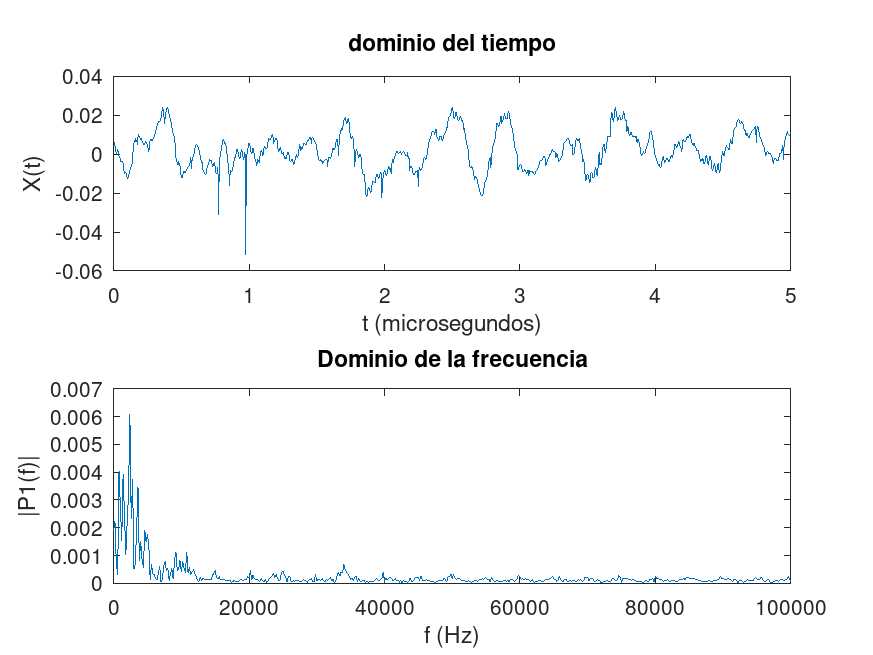
\includegraphics[width=\linewidth]{Dominios.png}
        Realizada con el Software Octave a partir de los datos de.
                \Cite{HUANG20181745}
        \label{Dominios}

	\end{figure}


El análisis en frecuencia suele ser más utilizado debido a que
la mayoría de las fallas poseen frecuencias características y, dado que en  el
análisis de frecuencia se descompone en frecuencias la señal, se facilita la
detección de fallas características, así mismo, la amplitud de la frecuencia es
directamente proporcional al nivel de la falla. Por lo tanto se obtiene un
espectro amplio del estado de la pieza.
Cabe resaltar que cuando las frecuencias son bajas o muy cercanas entre si,
se dificulta determinar e identificar alguna falla, suele suceder cuando se
estudia una falla o evento con frecuencia muy baja o muy cercana a la frecuencia
natural de la señal o elemento medido. En estos casos es mejor
usar un análisis en el dominio del tiempo que  facilita la
detección de las fallas.



\subsubsection{Herramienta Computacional}


Según \Cite{Herramienta}, una herramienta computacional puede ser definida  como
cualquier software,
sistema de integración, análisis o almacenamiento que  ayuda a los científicos
o usuarios a solucionar un problema específico en una determinada rama. Pueden
variar desde sistemas complejos como compiladores, algoritmos
e incluso sistemas operativos hasta herramientas como hojas de cálculos, sistemas
de oficina o medios de comunicación. Funcionan mediante la implementación de
técnicas y protocolos para solucionar problemas de forma iterativa o con una
secuencia de pasos concreta.

Siguiendo este orden de ideas, una gran cantidad de estas herramientas son
encontradas en la librería de información más grande del mundo, el Internet.
Todas comparten la peculiaridad de que son un \textbf{sistema} y,  por ende, pueden
ser accedidas con facilidad desde cualquier punto con un dispositivo capaz de
tener conexión a Internet y un navegador. Esta facilidad se debe a que un
\textbf{servidor} se encarga de hacer el procesamiento de la información y envía
el resultado con un formato específico, típicamente son  JSON, por \comillas{notación de
objeto de JavaScrip} el cual es un formato de texto sencillo para el intercambio de
datos, este se renderiza (proceso para generar una representación gráfica por
medio de programas informáticos) en una pagina Web.

\subsubsection{Sistema Web}

Los sistemas Web, de acuerdo a \cite{SistWeb1} y \cite{wiki:systemWeb}, o
también conocidos como aplicaciones Web son sistemas que
utilizan la tecnología Web y el Internet o Intranet para transmitir la
información y los
servicios a usuarios o otros sistemas/aplicaciones. Estos sistemas utilizan los
principios del hipertexto para renderizar la información en cualquier
navegador o \textbf{pagina Web} y el poder de los \textbf{servidores} para
almacenar y procesar la información. Por estas características son independientes
de cualquier plataforma o sistema operativo, además de  no requerir ningún
proceso de instalación, facilitando de esta forma el acceso, la gestión y la
rapidez de obtención de información.



\subsubsection*{Página Web}
Una página Web, como se explica en \cite{webpageMozila},  es un documento
accesible desde cualquier navegador con acceso
a Internet que puede incluir audio, vídeo, texto y sus diferentes
combinaciones.
Funciona al usar el protocolo HTTP, conocido usualmente como la Web, y una
estructura de hipertexto la cual permite redirigir, enlazar y estructurar el
contenido y lo hace fácilmente accesible desde un navegador Web.

Funciona gracias al protocolo HTTP, \comillas{Hypertext Transfer Protocol},
el cual es la base de cualquier intercambio de datos en la Web y un protocolo
de estructura cliente-servidor, esto implica que una petición de datos es
iniciada por el elemento que recibirá los datos (el cliente), normalmente un
navegador Web, y es cubierta por el elemento que envía los datos (el servidor).
Este protocolo comenzó siendo estático y dirigido usualmente a la transmisión de
texto pero se fue convirtiendo en más que eso y en la actualidad permite la
transferencia de documentos de todo tipo, scripts, vídeos, entre otros; a tal
punto que es fácilmente categorizado como el protocolo más usado en todo el
mundo, siendo incluso utilizado como sinónimo de Internet cuando es solo una
parte de él.

Debido a la invención de tecnologías como JavaScrip y AJAX hoy en día es
posible tener aplicaciones Web, que son programas junto a una interfaz gráfica,
que permite comunicarse con servidores que realizan la mayor parte del trabajo.
 Es posible el desarrollo de aplicaciones complejas que funcionen desde la
comodidad de dispositivos móviles. La Web permite, por tanto, facilidad a la hora
de transmitir información así como el poder acceder a cualquier contenido desde
cualquier dispositivo en cualquier momento.

La Web suele ser el método de acceso de muchas tecnologías y, si bien en la actualidad
el desarrollo Web usa el mismo estándar de tecnologías, el lado del servidor
contempla una variedad mucho más amplia, dado que cualquier aplicación que
pueda correr en un ordenador puede ser conectada a una interfaz Web. Teniendo
como limitante principal la latencia,  tiempo que tarda la información en viajar,
una interfaz Web es, para un usuario promedio, una solución cómoda y
accesible la cual  permite incluso  mayor comodidad y facilidad de acceso.


\subsubsection*{Servidor}

Un servidor Web, como lo define \Cite{servidor},  es un ordenador de propósito
específico que permite la
transición de datos a uno o múltiples clientes Web. Para esto, el dispositivo
debe de estar configurado para escuchar las solicitudes de los clientes en un
entorno red. Esto se logra mediante una aplicación externa o el uso de un
sistema operativo dedicado; almacena los archivos
necesarios para el procesamiento de información y los datos necesarios para
mostrarla, además, se encarga de distribuirla al usuario final.

Los servidores se suelen clasificar según su función y es común que cumplan más
de una función, o se encuentren más de un tipo en una red. Algunos de estos son
servidores de archivos, impresión, aplicaciones, DNS, \textbf{Web}, entre otros.
Actualmente, los servidores Web son los más abundantes en el mercado
y se caracterizan por alojar la información y los datos de los usuarios a través
de Internet o Intranet. Estos responden a las solicitudes de paginas Web u otros
servidores basados en esta tecnología.


\subsubsection{Interfaz de programación de aplicaciones (API)}
Interfaz de programación de aplicaciones es una forma de simplificar el diseño
de software al permitir el intercambio de información y funcionalidades de forma
rápida y segura. Como explica \cite{API} una API permite a las compañías y
desarrolladores abrir y expandir las informaciones y funcionalidades que poseen
con grupos externos de desarrolladores, compañeros de negocios e incluso departamentos
internos dentro de la misma compañía, esto permite separar los desarrollos y
trabajar de forma paralela ya que los desarrolladores no necesitan conocer la
implementación, simplemente la utilizan como interfaz para comunicarse con otros
productos y servicios.

Cabe resaltar que sin estas fuera imposible el desarrollo de muchas aplicaciones
populares. Una API funciona al ser un conjunto de normas que defines como se
comunicaran las computadoras o aplicaciones entre ellas, es decir, sirve como
una capa de abstracción entre el servidor y la aplicación.

\subsubsection{Modelo estadístico}

Un modelo estadístico, de acuerdo a \cite{modeloIBM}, es una representación
matemática que permite, mediante
ecuaciones, codificar información extraída de los datos y, de esta forma,
predecir el comportamiento de un sistema ante situaciones dadas. Funcionan
mediante  variables aleatorias, una o más variables de las cuales no
se tiene completa certeza de su valor o provienen de algún evento aleatorio.

Un modelo estadístico permite inferir ciertas características de un evento,
como qué tan probable es tal evento y cómo se distribuyen los valores de la
variable. Además se suele usar como primer paso en generar un modelo más
preciso o para la obtención de información cuando no se tiene suficiente,
es difícil su acceso o la naturaleza del
sistema es extremadamente compleja y dicha tarea es simplemente imposible.


\subsubsection{Lenguaje de programación}
Los lenguajes de programación pueden ser definidos, según \cite{ETAC} como
sistemas estructurados
que permiten a las personas o programadores interactuar y dar instrucciones a un
programa o software con la finalidad de lograr objetivos.

En la actualidad existen una gran cantidad de lenguajes de programación, algunos
desarrollados en la antigüedad que todavía desarrollan un papel importante en
los sistemas, como lo son C, C++, Java y otros más modernos como lo pueden ser
Go, Rust y Python.

Como se explica en \cite{javaTpoint}
Los lenguajes de programación suelen ser clasificados en bajo nivel y alto nivel,
haciendo referencia a la necesidad de un compilador o intérprete para poder ser
ejecutado por la computadora, siendo los de bajo nivel lenguaje de máquina o
ensamblador y los de alto nivel los lenguajes comúnmente conocidos, como
Python, Java, JavaScript, PHP, C++, Objective C, Cobol, Perl, Pascal, LISP,
FORTRAN, Go y Swift. Estos lenguajes de alto nivel se pueden subdividir
de acuerdo a la necesidad de un compilador (C,C++,Go, etc.) o de un intérprete
(Python, JavaScript, Ruby, etc.) en \cite{LenguajesCompiladosEInterpretados}, se
puede leer más de esto. Asimismo, existe otra pequeña subdivisión en el ``tipado"
del lenguaje, que es la necesidad de especificar el tipo de valor que una
variable o constante puede tomar, siendo estas posibilidades un tipado fuerte,
medio o débil, también llamados dinámico (débil) o estático (fuerte).


\subsubsection{Go}
Go es un lenguaje de programación creado en 2007 en google, específicamente por
Robert Griesemer, Rob Pike y Ken Thompson, su sintaxis es similar a la del lenguaje
C y tiende a ser dinámico como Python pero con un rendimiento equiparable a los
de C o C++. Como se especifica en su pagina y documentación oficial
\cite{GolangDocumentacion}: Go es un proyecto de código abierto (open source)
para hacer a los programadores más productivos, es un lenguaje expresivo, conciso,
limpio y eficiente con mecanismos de concurrencia (paralelismo) que permiten fácilmente
obtener el máximo rendimiento posible de las máquinas multinucleo y redes de máquinas
actuales, mientras permite una programación flexible y modular, además de un compilado
rápido con un recolector de basura (el lenguaje se encarga de liberar memoria
no utilizada).
Es un lenguaje compilado rápido y con tipado estático (las variables y sus tipos tienen que
ser definidos con anterioridad) que se siente como un lenguaje interpretado y
con tipado dinámico (variables modificables sin tipo definido, más sencillo de
escribir el código pero menos estructurado).

Adicional a esto, este lenguaje tiene un ecosistema de comunidades, librerías y
herramientas en constante crecimiento que facilitan el aprendizaje y el desarrollo
de código.

\subsubsection{Fyne}

Fyne es una de las librerías (conjunto de herramientas o paquete) más utilizado
en Go para el desarrollo de GUI, como se indica en su pagina oficial \cite{fyne}
el conjunto de herramientas de Fyne es una herramienta fácil de aprender, gratuita
y de código abierto (open source) que permite la creación de aplicaciones gráficas
para escritorios, teléfonos y más. Combina el poder y la simplicidad del lenguaje
Go con una cuidadosamente creada librería de widgets (miniaplicaciones o herramientas)
que hacen ahora más fácil que nunca la construcción de aplicaciones y su despliegue
a producción en todas las plataformas (sistemas operativos, ios, linux, windows, etc.)
y tiendas (windows store, google play, etc.).

\subsubsection{HTML}

HTML no es considerado un lenguaje de programación propiamente dicho por su
incapacidad de realizar acciones de lógica o aritmética, más específicamente y
de acuerdo a \cite{HTML},
es un lenguaje de enmaquetado (una forma de escritura que utiliza elementos
sintácticos para dar forma y estructura a la información escrita posteriormente
a un proceso de  compilación o interpretación por la máquina, otros ejemplos son
Latex y Markdown), específicamente un lenguaje de enmaquetado de hipertexto y es
el bloque más básico para la Web ya que define y estructura el contenido de la
misma.

``Hipertexto"\  se refiere a los enlaces que se utilizan para conectar la pagina
web con otras partes, ya sean de la misma pagina o paginas externas a la misma.
Estos enlaces son fundamentales en la Web ya que permiten la actualización y el
entrelazamiento de las paginas creadas por otras personas, esto permite
una participación activa el la\  ``World Wide Web".

HTML usa ``etiquetas"\  para dar información adicional  el texto, las imágenes,
el contenido y permitir
una correcta muestra del contenido, estos elementos sintaxicos son por ejemplo:
 <head>, <title>, <body>, <header>, <footer>, <article>, <section>, <p>, <div>,
 <span>, <img>, <aside>, <audio>, <canvas>, <datalist>, <details>, <embed>,
 <nav>, <output>, <progress>, <video>, <ul>, <ol>, <li>, entre otros.

 De esta forma, el mismo texto entre etiquetas distintas va a tener características
 visuales distintas, por ejemplo, <h1>Algo<h1> es un título, negritas y tamaño de
 fuente muy superior a <p>Algo<p> que sería un párrafo.


\subsubsection{CSS}

CSS al igual que HTML no es considerado un lenguaje de programación, por las mismas
razones, en cambio, como se describe en \cite{CSS} es una hoja de estilos en cascada,
un lenguaje utilizado para describir y dar estilo a documentos escritos en HTML o
XML, Esto lo consigue al describir como los elementos deberían ser mostrados en la
pantalla, papel, habla u otra tipo de multimedia.

Dado estas características CSS es una parte fundamental en el desarrollo Web, ya
sea en su versión para o con la inclusión de frameworks o librerías como lo son
Bootstrap o TailWind CSS.

Funciona mediante la especificación y modificación de las características en
entornos, etiquetas o elementos únicos, mediante identificadores, de un entorno
HTML o XML y por esto permite la modificación de los atributos.
Usualmente, en términos Web, se modifican tamaños de fuente, peso de la misma,
color de fondo o de fuente, márgenes, espaciado interno (padding), centrado,
entre otras cosas, y mediante la fijación de estas características a atributos
particulares se puede desarrollar un entorno gráfico completo, animaciones y
transiciones.

\subsubsection{JavaScript}

Como se describe en \cite{JavaScript}, este lenguaje de programación es liviano e
interpretado, débilmente tipado y es comúnmente conocido como el lenguaje estándar
de los scripts en las paginas Webs; sin embargo, también puede ser utilizado en
otros ambientes como a nivel de servidor y en aplicaciones multiplataforma.
JavaScript es un lenguaje basado en prototipos, multiparadigma, dinámico y de
ejecución en un silo hilo (no aprovecha la paralelización de los múltiples
núcleos) y soporta todo tipo de estilo de programación.

Sus estándares han ido evolucionando con el tiempo y son conocidos como
`` ECMAScript Language Specification"; comúnmente JavaScript corre del lado del
cliente y es utilizado para diseñar como las paginas web se ven o se comportan
ante algún evento especifico.

Al ser un lenguaje tan popular y común, posee una gran comunidad y una cantidad
muy significativa de ``Frameworks"  y librerías, facilitando su aprendizaje
y maximizando la cantidad de cosas que permite hacer. Entre las más conocidas
están: Node.js para el servidor, React, Angular y Vue para el cliente, además
existen librerías como JQuerry que facilitan el lenguaje.

\subsubsection{React}

React es una librería de JavaScript de código abierto diseñada por facebook y
lanzada por primera vez en 2013, como dice su documentación oficial \cite{React}
está diseñada para la construcción de interfaces de usuario, tiene una filosofía
de pagina única (singlepage) pero puede ser utilizada para desarrollar aplicaciones
de múltiples paginas. Esta librería tiene la característica de ser declarativa
y basada en componentes.

Como se mencionó anteriormente, React hace sencillo la creación de interfaces
de usuario al permitir la combinación de JavaScript con XML-HTML en ``jsx"\  dando
la posibilidad de devolver y renderizar HTML desde funciones con componentes
lógicos. Además, es completamente modular por lo que se pueden desarrollar
individualmente los elementos de la interfaz y juntarlos con total facilidad,
estos elementos son llamados componentes y utilizan todas las propiedades de
JavaScript y la manipulación del DOM (Document Object Model) para mostrar
y actualizar la información cuando es necesario.


\subsubsection{Python}

En su página oficial, específicamente en sus preguntas frecuentes
\cite{pythonDocs} se especifica que Python es un lenguaje de programación
interpretado, interactivo y orientado a objetos, este soporta muchos paradigmas
además del orientado a objetos, como lo son el procedimental y el funcional.
Python incorpora funcionalidades como módulos, excepciones, un tipado dinámico
y un muy alto nivel de dinamismo en los tipos de datos y clases, asimismo,
combina un poder computacional bastante alto con una muy clara sintaxis,
librerías, sistemas y compatibilidad con todos los sistemas operativos, además
de una facilidad para extenderse a los lenguajes C o C++.

Cabe resaltar que Python es completamente gratuito y tiene una gran capacidad,
dada su gran cantidad de librerías y frameworks, para cumplir muchas tareas,
como lo son estadística, sistemas webs, ciencia de datos entre otros.

\subsubsection{Django}

Django es un framework web de alto nivel de Python el cual fomenta un
desarrollo rápido, limpio y pragmático. Como se especifica en su documentación
oficial,
\cite{DjangoDoc} Fue creado para desarrolladores con experiencia que necesitan
un desarrollo rápido y completo en un proyecto web, con la finalidad de
permitir al programador desarrollar la aplicación propiamente dicha, es
completamente gratuito y de código libre.

Entre las características de Django son su gran velocidad para el diseño, gran
cantidad de extras y tareas adicionales fácilmente configurables
(autenticación, administración, etc.), seguridad (previene errores comunes
como SQL injection y  cross-site scripting-requests), versatilidad y facilidad
de escalabilidad.

Cabe destacar que Django permite la inclusión de librerías de Python para
cualquier ámbito y existen algunas específicamente diseñadas para facilitar el
desarrollo con este framework, por ejemplo Django rest framework, para la
creación de APIs desde el servidor de Django  y Django-cors-headers que permite
modificar y controlar el acceso de solicitudes a APIs desde clientes.

\subsubsection{Numpy}

Numpy es un paquete-extensión de Python diseñado para la computación
científica. Como se explica en su documentación oficial \cite{Numpy} es una
herramienta de computación numérica que ofrece una gran cantidad de  funciones
matemáticas, generación de números aleatorios, rutinas algebraicas de álgebra
lineal, transformadas de Fourier, el tratado de arreglos N-dimensionales,
vectorización e indexación de los mismos, todo esto a un gran rendimiento y una
facilidad notable de su uso . Además de todo esto, esta es una herramienta
gratuita de código abierto.

\subsubsection{Pandas}

Pandas es otra herramienta dedicada al cálculo numérico, es una herramienta
rápida, poderosa, flexible y de fácil utilización, además de código abierto,
utilizada para el análisis y la manipulación de datos, es creada en Python.
Entre sus características destacan su velocidad y eficiencia con objetos de
tipo DataFrame para la manipulación de la información, sus herramientas para la
lectura y escritura de información en distintos formatos, entre los cuales
destacan los formatos CSV, Excel, SQL DataBase y el HDF5, facilidad para la
mutabilidad, alineamiento, filtración y eliminación, inserción y separación de
datos, y una muy alta optimización con puntos de código críticos escritos en
Cython o C. Además de esto, otras características adicionales son expuestas en
su documentación oficial \cite{PandasDocs}

\subsubsection{SciPy}
SciPy es una librería-colección de algoritmos para la computación científica en
Python, como se explica en su sitio oficial \cite{Scipy}, esta desarrollado de
forma abierta en GitHub a traves del consenso y el trabajo de la comunidad
científica de Python y de la comunidad de SciPy. Esta herramienta provee estructuras
de datos y
algoritmos para optimización, integración, interpolación, problemas algebraicos,
ecuaciones, ecuaciones diferenciales, estadística, entre otros. Esta escrita
en lenguajes de medio-bajo nivel, como lo son Fortran, C y C++, haciendo sus
implementaciones bastante optimizadas y permitiendo el uso de código compilado
con la flexibilidad y facilidad de uso de Python.

\subsubsection{FastApi}
\cite{FastApi} define FastApi como un framework moderno y rápido, con alto
rendimiento, diseñado para
la construcción de APIs web en Python, tiene una versión mínima de 3.6. Sus
características principales son:

\begin{itemize}
    \item velocidad, equiparable con Node.js y Go haciéndolo
uno de los frameworks de Python mas rápidos actualmente.
    \item velocidad de escritura, permitiendo alcanzar un aumento en el desarrollo
        de hasta un 300\%.
    \item Facilidad, esta desarrollado para ser intuitivo, fácil, permitiendo
        reutilización y a su vez eliminando hasta un 40\% de los errores ( ``bugs")
        inducidos por humanos.
    \item Utiliza estándares de código abierto como lo son ``OpenApi"" y ``JSON Schema"".
\end{itemize}

\subsubsection{Octave}
Octave es un software originalmente escrito por John W.Eaton y muchos otros,
esto es debido a que es un lenguaje gratuito y constantemente incorpora
funciones o correcciones hechas por la comunidad. Como se especifica en su
documentación oficial \cite{octave}, es un lenguaje de programación de alto
nivel, orientado primordialmente a la realización de cálculos numéricos.
Permite el uso de una interfaz  o la terminal para resolver ecuaciones
lineales, no lineales, problemas numéricos además de conversiones y
transformadas matemáticas. Es completamente compatible con el lenguaje Matlab y
además puede ser utilizado como un lenguaje orientado a procesos.

Cabe resaltar que octave posee una gran gama de librerías o módulos escritos en
C++, C, Fortran entre otros lenguajes, y es completamente gratuito y
redistribuible.


\subsection{Git}
Es un software de control de versiones diseñado por Linus Torvalds pensado para
la confiabilidad y compatibilidad del mantenimiento de versiones de aplicaciones
especialmente útil cuando estas tienen un gran numero de versiones y archivos.
Como explica \cite{Git}, Git es un sistema de control de versiones distribuido,
gratuito y de código abierto, diseñado para manejar eficientemente tanto pequeños
como grandes proyectos de forma rápida y eficiente. Se diferencia de otros sistemas
por características como ramificaciones locales baratas, en términos computacionales
espacio y velocidad, múltiples flujos de trabajo en áreas de ensamblaje convenientes
(Permite trabajar tanto en clientes gráficos como en la terminal).

\subsection{GitHub}
GitHub es una plataforma para el montaje de  código y el control de versiones
basada en Git. Se utiliza para la creación de código fuentes ya que permite y
facilita la interconexión entre los programadores, como se explica en \cite{github}
GitHub  permite incrementar la velocidad del desarrollador, además de asegurar
cada paso, automatizar los espacios y flujos de trabajo, facilitando de esta
forma los patrones de desarrollo e integración continua y permitiendo la creación
de equipos de trabajo sin el impedimento de la ubicación geográfica.

\subsubsection{Digital ocean}

    \endgroup
    %
\subsection{Glosario}

\begin{itemize}
    \item motor electrico
    \item estator
    \item rotor
    \item torque
    \item potencia
    \item rodamiento
    \item Transferencia de potencia
    \item vibracion
    \item sensor
    \item adquisicion de datos
    \item ancho de banda
    \item acelerometro
    \item aceleracion
    \item posicion
    \item velocidad
    \item frecuencia
    \item acelerometro capacitivo
    \item acelerometro pizoelectrico
    \item acelerometro pizorresistivo
    \item Sistema de segundo orden
    \item dispositivo microelectromecánicos
    \item masa sísmica
    \item amortiguamiento
    \item Circuitos Integrados
    \item galgas extensiométricas
    \item rango dinamico
    \item voltajes DC
    \item voltajes AC
    \item ruido
    \item linealidad
    \item ancho de banda
    \item cristal pizoelectrico
    \item amplitud
    \item nivel offset
    \item señal analogica
    \item señal digital
    \item convertidor Analógico-Digital
    \item Dominio del tiempo
    \item Dominio de la frecuencia
    \item transformada de fourier
    \item componentes de una señal|
    \item Frecuencia natural
    \item herramienta computacional
    \item servidor
    \item pagina web
    \item Json
    \item Hipertexto
    \item internet
    \item intranet
    \item Web
    \item Pagina web
    \item Servidor
    \item javascript
    \item AJAX
    \item latencia
    \item Variable aleatoria
    \item Modelo estadistico
\end{itemize}


    %Faltan mas teorias, de lo usado y tal vez otro antescedente

    %Cuadros o graficas muy breve, que contenga la informacion
    %y dudas y permita recordar

%***************************************************
%**********  Capitulo 3  ***************************
%***************************************************
	\newpage
    \begingroup
    \let\clearpage\relax

    % naturaleza de la investigacion, Tipo de investigacion
	\thispagestyle{empty}

\section{MARCO METODOLÓGICO}

Como fue explicado en el primer capítulo, se pretende hacer una herramienta
computacional para el análisis de la vibración en motores eléctricos alimentada
mediante datos de una simulación digital. Partiendo de esto, se comenzará
con la definición de los siguientes aspectos.

\subsection{NATURALEZA DE LA INVESTIGACIÓN}

El presente trabajo es clasificado como Proyecto Especial, puesto que según
\textcite{Hernandez} lleva~a:

\begin{center}
    \parbox[ht]{13.5 cm}{Trabajos que lleven a creaciones tangibles,
    susceptibles de ser utilizadas como soluciones a problemas demostrados, o
    que respondan a necesidades e intereses de tipo cultural. Se incluyen en
    esta categoría los trabajos de elaboración de libros de texto y de
    materiales de apoyo educativo, el desarrollo de software, prototipos y de
    productos tecnológicos en general, así como también los de creación
    literaria y artística.}
\end{center}


\subsection{TIPO DE INVESTIGACIÓN}

De acuerdo con la clasificación el tipo de investigación de este trabajo se
cataloga como investigación aplicada, puesto que "persigue fines inmediatos y
concretos a través de la búsqueda de un nuevo conocimiento técnico con aplicación
inmediata a un problema determinado"\ \textcite{Velez}.

\subsection{FASES DE LA INVESTIGACIÓN}

En función de los objetivos específicos, se pueden definir las fases que conforman
la investigación:

\subsubsection{Definición de los requerimientos de usuario}
Esta fase tiene relación directa con la concepción del proyecto ya que fue el
planteamiento de los problemas y posibles soluciones, separación de vistas,
mecanismos de análisis, entre otros. Sin una concepción compleja de las estructuras
de datos y los lenguajes necesarios para elaborarla.
Como en todo proyecto, esta fase requirió de la interacción con el cliente (ingeniero
mecánico que propuso la idea) con la finalidad de puntualizar los requerimientos
mínimos necesarios para obtener una aplicación viable.

De esta manera, la primera fase ha constado de las siguientes actividades:

\begin{itemize}
    \item Selección de la cantidad de vistas óptimas para facilitar el estudio
        y el monitoreo de la planta, siendo esto decidido a 3, una vista
        \textbf{general} del estado de los motores en la planta, una
        \textbf{especifica} en donde se observa el comportamiento de un motor,
        una \textbf{exhaustiva} que añada información a la especifica, gráfica en
        el dominio de la frecuencia, agregada para mejorar la experiencia de
        usuario, por la demora necesaria para generar este estudio.
    %
    \item Definición de la estructura mínima necesaria para poder evaluar un
        motor, en términos de evolución histórica de la vibración, a base de
        una tabla histórica o gráfica (histórica).
    %
    \item Definición del tipo de transformada de Fourier a graficar para el
        análisis exhaustivo (por gustos y costumbres en la industria).
    %
    \item Entrega de una base de datos histórica con mediciones reales y esporádicas
        del estado de los motores en una fabrica.
    %
    \item Especificación de los parámetros a considerar para determinar un nivel
        básico del estado de un motor, en términos de velocidad y aceleración.
        Se debe resaltar que estos valores difieren de los establecidos a nivel
        teórico y recomendado en los estándares por factores inherentes a las
        empresas (malas instalaciones,
        utilización de bases artesanales, políticas de daños mínimos) los cuales
        amplían los rangos teóricos.
    %
    \item Selección de las unidades en las que se tomaran las medidas, siguiendo
        estándares, y siendo $\frac{mm}{s}(rms)$ para la velocidad y $g$ para la
        aceleración.
\end{itemize}

Es importante recalcar el hecho que los parámetros utilizados tanto
para el establecimiento de niveles de daño en el modelo estadístico como
en la vista general para distinguir el estado de los motores, son el resultado
empírico asociados a años de estudios del comportamiento de los motores en la
planta utilizada. Esto se tomo en consideración al momento del diseño y se puede
modificar, vía modificación de constantes en el código, los rangos de valores
en velocidad y vibración adecuados a los estándares de cada planta o ingeniero
que utilice el sistema.

\subsubsection{Revisión documental}
Relacionada parcialmente con los primeros dos objetivos de la investigación,
se baso en los estudios necesarios para poder tomar la decisión del tipo de modelo
y lenguajes a utilizar, el planteamiento de requerimientos para los
lenguajes, dada la gran variedad de posibilidades disponibles para las distintas
tareas a realizar; de esta forma, se pueden enumerar las siguientes actividades
realizadas:

\begin{itemize}
    \item Recolección de información de diversos lenguajes de programación.
    \item Estudio de estadística y los distintos modelos y distribuciones existentes.
    \item Estructurar los criterios y requerimientos mínimos para poder seleccionar
        las herramientas a utilizar.
\end{itemize}

\subsubsection{Análisis de la información}
Todavía una fase previa a la implementación pero relacionada al primer objetivo
de la investigación. Se procedió a analizar la información en la bases de datos,
comparar con los requerimientos mínimos por el cliente y estructurar mas detalladamente
tanto la nueva base de datos (creada posteriormente en MongoDB), los parámetros
necesarios para el modelo estadístico y la selección del tipo, orientado a una
distribución de probabilidad. Asimismo, se tomaron decisiones conforme a los
lenguajes utilizados y la estructura, de microservicios, que se utiliza en el
desarrollo. De esta forma, se distinguen los siguientes puntos en esta fase:

\begin{itemize}
    \item Organización de la información recolectada.
    \item Toma de decisión de los lenguajes y herramientas a utilizar, basada
        en los criterios previamente establecidos.
    \item Estructuración de los modelos para la base de datos.
    \item Justificación de las decisiones tomadas.
    \item Estructuración y separación de las tareas a realizar por los distintos
        microservicios (sensorica, Web, BBDD).
\end{itemize}

\subsubsection{Diseño del modelo estadístico}
Corresponde al segundo objetivo del trabajo pero guarda relación con los
objetivos 3 y 4. Se utilizaron técnicas de exploración de data para la
selección de las variables de interés así como la formulación de hipótesis y se
usaron pruebas estadísticas para seleccionar las distribuciones de probabilidad
que mejor modelan las variables de interés. Se realizaron las siguientes
tareas:

\begin{itemize}
    \item Limpieza de los datos.
    \item Análisis exploratorio de la data.
    \item Cálculo de estadísticos de interés.
    \item Cálculo de pruebas de bondad de ajuste para cada variable de interés.
    \item Selección de la distribuciones que mejor modelan cada variable.
\end{itemize}

\subsubsection{Diseño de las vistas para mostrar la información}
Este apartado guarda relación con los objetivos 5 y 6. Se trabajo en la
estructuración y diseño gráfico de las vistas, además de las funcionalidades
implementadas para poder ser creada la pagina Web. Las tareas realizadas
fueron las siguientes:

\begin{itemize}
    \item Toma de decisión en utilizar una aproximación multipagina (multipage app).
    \item Diseño básico, barra de navegación, encabezado y pie de pagina.
    \item Diseño de la vista General y su funcionalidad.
    \item Diseño de la vista Especifica y su funcionalidad.
    \item Diseño de la vista Exhaustiva y su funcionalidad.
\end{itemize}

\subsubsection{Implementación}
Dada la gran cantidad de tareas a desarrollar, la implementación se subdivide
en un gran grupo de tareas, con la finalidad de cumplir los objetivos 2,3,4,5,6
estas divisiones, y subdivisiones, pueden ser expresada de la siguiente forma:

\begin{itemize}
        \item Generación del modelo estadístico:
    \begin{enumerate}
        \item Inspección manual de la data.
        \item Limpieza de las variables de interés.
        \item Elaboración de histogramas para observar la distribución de los datos.
        \item Seleccionadas las variables velocidad horizontal, velocidad
            vertical y aceleración como variables para el modelo.
        \item Cálculo de correlación entre variables.
        \item Cambio de variables para reducir la correlación entre velocidad
            horizontal y velocidad vertical.
        \item Búsqueda de distribuciones que mejor modelan la data utilizando
            múltiples pruebas de Kolmogorov-Smirnov.
        \item Selección de distribuciones de Burr tipo III para modelar la
            magnitud de la velocidad y aceleración y distribución normal para
            modelar el ángulo.
        \item Calculo de parámetros de las diferentes distribuciones. Creación
            de API en FastAPI para servir los datos.
        \item Conexión de la API con el microservicio de Go.
    \end{enumerate}

    \item Elaboración de la base de datos:
        \begin{enumerate}
            \item Registro y creación del cluster en MongoDB Atlas.
            \item Creación de la base de datos ``tesis"\  y las colecciones
                ``MotorData"\  y ``MotoresInDB".
            \item Llenado mediante el servidor de sensorica.
        \end{enumerate}

    \item Microservicios de sensorica:
        \begin{enumerate}
            \item Creación de las estructuras de datos necesarias para manejar
                la comunicación con MongoDB.
            \item Obtención de un certificado y TLS/SSL.
            \item Creación del servidor Https.
            \item Creación de un cliente de sensorica, para facilitar la emulación
                de los sensores
            \item Implementación de las conexiones bidireccionales para el trafico
                de información.
            \item Creación del punto de conexión ``/sensormessage" para permitir
                la conexión de múltiples clientes y recibir la información.
            \item Creación del punto de conexión ``/exhaustive?idMotor\=identificador"
                para poder enviar la información de la vista exhaustiva.
            \item Intercomunicaciones internas en el servidor para poder comunicar,
                solicitar y verificar información entre los dos puntos de conexión.
            \item Verificaciones de seguridad y conexiones.
        \end{enumerate}

    \item Análisis en frecuencia:
        \begin{enumerate}
                \item Falta escribir
        \end{enumerate}

    \item Servidor Web:
        \begin{enumerate}
            \item Configuración para el envió de información estática
                (HTML, CSS, Js, imágenes).
            \item Creación del punto de conexión ``/" para la vista general.
            \item Creación del punto de conexión ``/especifica?IdMotor\= identificador"
                para la vista especifica.
            \item Creación del punto de conexión ``/exhaustiva?IdMotor\=identificador"
                para la vista exhaustiva.
            \item Creación de gráficas históricas.
            \item Solicitud de información y análisis en frecuencia, creación de
                la gráfica de frecuencia.
            \item Establecimientos de los puntos de conexión para las APIs que
                suministran las informaciones necesarias para las vistas (
                uno para cada vista).
        \end{enumerate}

    \item Muestreo de información, mediante las vistas:
        \begin{enumerate}
            \item Solicitudes de información a las APIs (fetch).
            \item Configuración de los valores y los niveles de daño.
            \item Establecimiento del motor svg con colores dependiendo del nivel
                de daño.
            \item Mecanismo de paginación y búsqueda para hacer mas fácil y agradable
                la UI.
            \item Creación de la vista general.
            \item Implementación de la tabla y la funcionalidad para exportar a
                excel.
            \item Solicitud y establecimiento de las imágenes-gráficas.
            \item Implementación de la vista especifica.
            \item Implementación de la vista exhaustiva.
            \item Diseño y estilizado mediante CSS.
        \end{enumerate}

    \item Interconexiones:
        \begin{enumerate}
            \item Interconexiones entre cliente y servidor de sensorica, mediante
                Http2 para poder establecer una comunicación bidireccional (full dúplex).
            \item Interconexión entre servidor de sensorica y API de modelo
                estadístico para información normal, grupo de 10
                mediciones de velocidad y aceleración por cada sensor.
            \item Interconexión entre servidor de sensorica y API del modelo
                estadístico para información exhaustiva, grupo de 1K de mediciones
                de aceleraciones, por sensor registrado al motor.
            \item Interconexiones entre el servidor de sensorica y la base de datos
                (MongoDB Atlas).
            \item Interconexiones entre el servidor Web y la base de datos (MongoDB Atlas).
            \item Interconexión entre servidor Web y servidor de sensorica, para
                solicitar la vista información asociada a la vista exhaustiva.
            \item Interconexión entre cliente Web y servidor Web para obtener
                información de archivos estáticos.
            \item Interconexión entre cliente Web y APIs del servidor Web para
                obtener la información referente a las vistas general, especifica
                y exhaustiva. Una interconexión y una API para cada vista.
        \end{enumerate}
\end{itemize}


\subsubsection{Comprobar los resultados}
Esta fase hace referencia al ultimo objetivo de la investigación: Comprobar los
resultados de la herramienta de análisis. Dada la extensión de la herramienta,
estas pruebas se pueden desglosar en dos niveles, resultados finales (evaluación
del análisis de la herramienta) y pruebas técnicas (también llamado testing).
Esto da origen a las siguientes tareas:

\begin{itemize}
    \item Testing: La elaboración modular del sistema permite  corroborar su
        funcionamiento de múltiples formas, dado que unas pruebas automatizadas
        escapan de esta investigación (por factores de tiempo y cantidad de pruebas
        y complejidad de las mismas a nivel de código) se toman pruebas manuales
        de sistemas e interconexión entre los mismos:
        \begin{enumerate}
            \item Prueba de no unicidad de la información, al haber múltiples
                clientes de sensorica enviando información sobre el mismo motor.
            \item Prueba de falla en la conexión de la base de datos.
            \item Prueba de solicitud de vista exhaustiva a un motor sin conexión
                establecida.
            \item Prueba de petición no completada en el cliente Web,
            información invalida (motor no existente) o error del servidor.
        \end{enumerate}

    \item Evaluación de resultados:
        \begin{enumerate}
            \item Corroboración del análisis en nivel de daño básico (vista general)
                que se ajuste a los parámetros requeridos por el cliente.
            \item Corroboración de las gráficas históricas.
            \item Corroboración de la gráfica de la transformada de Fourier.
        \end{enumerate}
\end{itemize}




    %Procedimiento de recoleccion de datos e informacion
    %Fases de la investigacion

    
\subsection{METODOLOGÍA}
\subsubsection{Metodología de desarrollo de software}

Para la implementación de los distintos sistemas que componen la herramienta
computacional propuesta, se necesitar seguir una metodología de diseño de
software. Como la herramienta se clasifica como una aplicación Web, las
metodologías utilizadas en el desarrollo de este tipo aplicaciones son
aplicables a este trabajo.

Las aplicaciones Web cuentan con muchas similitudes a las de aplicaciones de
computadores personales, sin embargo, una de sus principales diferencias es que
estas están en un estado de constante cambio por lo tanto
se pierde la noción de versiones, los cambios toman efectos de forma inmediata
y de forma gradual. Esta diferencia es producto de que su función principal es
la de transmitir información. Como esta información cambia de forma constante
los requisitos de la aplicación suelen también ser variables. Todo esto unido
al hecho de que los cambios en la aplicación pueden realizarse con la
menor fricción posible, los cambios se pueden observar al volver a cargar la
página, hace que este tipo de aplicación  exista en un estado de evolución
continua. Según \textcite{pressman2002}\  la evolución constante de las aplicaciones
Web puede ser comparada con la jardinería, se hace un trabajo inicial el cual
seria equivalente a sembrar un jardín y una vez se tenga el sitio implementado,
se debe realizar el trabajo de mantenerlo que seria equivalente a regar y
abonar las plantas.

Debido a lo presentado anteriormente, para le elaboración de los diferentes
componentes de la herramienta se realizó un desarrollo de forma continua,
en donde la aplicación tendrá la capacidad de evolucionar si algún día
cambian los requisitos de la misma. Para esto se utilizó la ayuda de
\textbf{Git} como sistema de control de versiones, lo cual permitiría integrar
los diferentes cambios de forma mas eficaz y facilitar la cooperación durante
el desarrollo de la aplicación. Para la elaboración de los diferentes
componentes se usa también un proceso iterativo, cada vez que se implemente
un componente se comprueba el funcionamiento del mismo y se corrige, de ser
necesario.

Este modelo de implementación posee una estructura muy marcada, la cual se adapta
a las metas, usuarios finales y a la filosofía de navegación que se elija.
Según \textcite{pressman2002} esta se puede desglosar como:

\begin{itemize}
    \item Diseño arquitectónico, el cual consiste en la definición de la
        estructura global, las plantillas y parte del patrón de diseño que se
        utilice para estructurar la red. Específicamente, se trata de cimentar
        las bases para facilitar la creación del contenido y se estructura la
        forma de navegación por el sistema, además de los componentes que la
        integren.

    \item Diseño de navegación, en esta fase se eligen las rutas de navegación
        que permiten el acceso al contenido, además, se hacen las distinciones
        con respecto a los  usuarios que accedan a la red y,
        por ende, las funcionalidades y/o permisos a los que tendrán acceso.

    \item Diseño de la interfaz, se refiere al diseño gráfico, estético y a
        las facilidades que se le dan a los usuarios, dado que esta es la primera
        impresión que se da, puede significar la diferencia entre el uso o no de
        la aplicación.

    \item Cabe destacar que, en la actualidad, se consideran mas fases que las
        mencionadas por Pressman, las dos mas resaltantes son la
        \textbf{Fase de programación} y la \textbf{Fase de Testeo}, aunque la
        última es nombrada como un proceso posterior al desarrollo. Estas dos
        fases son consideradas en la actualidad dados los constantes requerimientos
        de implementaciones adicionales o modificaciones a las ya existentes.
        Para permitir la integración de la mismas sin exponerse al colapso del
        sistema, se suelen utilizar \textbf{test} automatizados los cuales deben
        ser diseñados e implementados.

\end{itemize}

	
\subsection{RECURSOS}
\begin{itemize}	
	\item Computadoras portátiles.
	\item Documentación.
	\item Base de datos de la vibración en motores eléctricos.
\end{itemize}	
	%
\subsection{CRONOGRAMA DE ACTIVIDADES}

    Las actividades a realizar son las expuestas en la figura
    \ref{cronograma2}, y están pautadas para un
    lapso total de aproximadamente 13 semanas donde se planean 10 semanas de
    implementación:

%		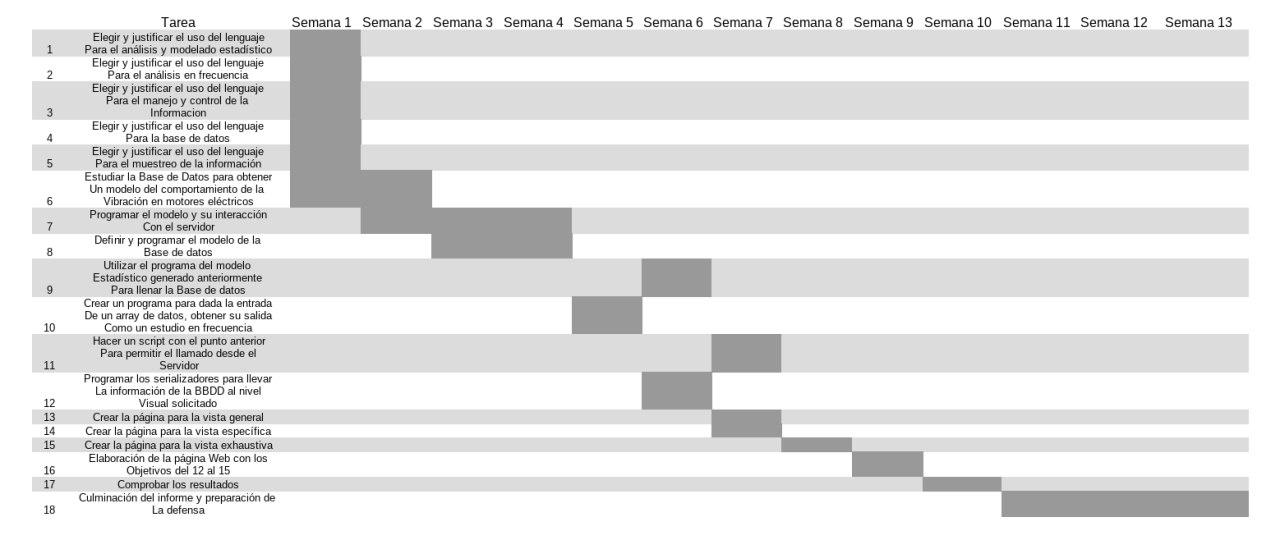
\includegraphics[trim= 2.5cm 0 -75 0,clip, width=1.2\linewidth  ]{diagrama_grant.jpg}
    \begin{figure}[htb]
		\centering
        \caption{Cronograma de actividades.}
		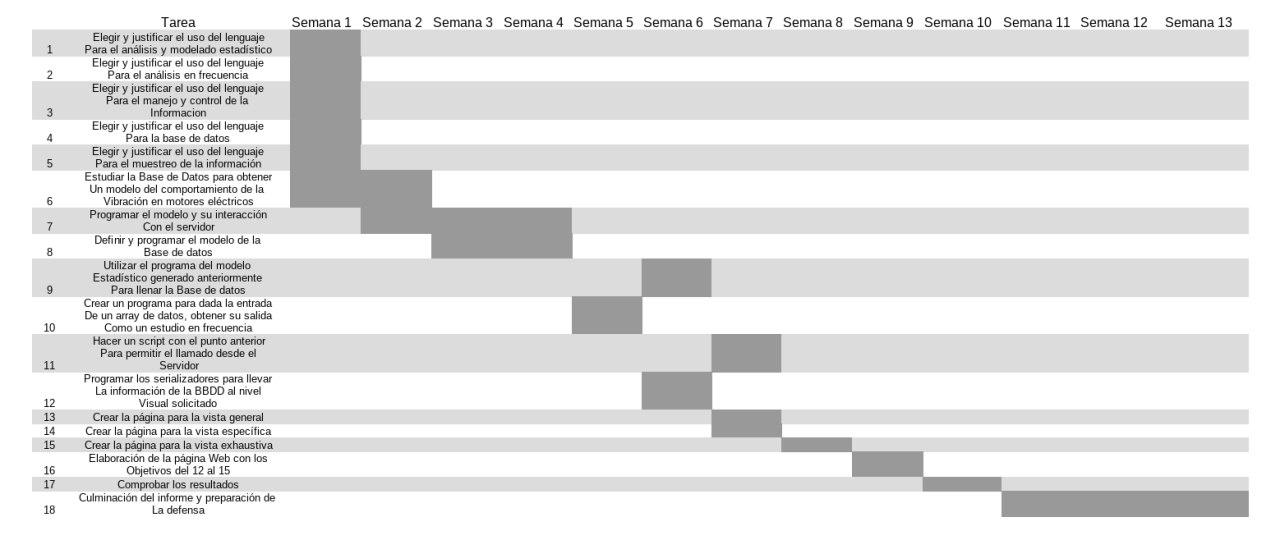
\includegraphics[ width=1.2\pdfpagewidth ,angle=270 ]{diagrama_grant.jpg}
		\label{cronograma2}
	\end{figure}



    \endgroup


%***************************************************
%**********  Capitulo 4  ***************************
%***************************************************
	\newpage
    \begingroup
    \let\clearpage\relax

    \thispagestyle{empty}

\section{ANÁLISIS Y DISCUSIÓN DE RESULTADOS}

\subsection{PROCEDIMIENTO DE RECOLECCIÓN DE INFORMACIÓN}
Esta parte del proyecto es bastante extensa así que debe de ser dividida en dos
categorías, investigación de campo e investigación documental.

La investigación de campo, según \textcite{MetodologiaInvestigacion}
es aquella que consiste en la recolección de datos directamente de los sujetos
investigados, o de la realidad donde ocurren los hechos,
sin manipular o controlar variable alguna, es decir, el investigador obtiene la
información pero no altera las  condiciones existentes. De allí su carácter de
investigación no experimental.

De esta forma, análisis de campo juega un rol importantísimo para obtener la
información y los requerimientos mínimos para el diseño de la interfaz de usuario
y del modelo estadísticos.

Asimismo, la investigación documental, según \textcite{MetodologiaInvestigacion}
es un proceso
basado en la búsqueda, recuperación, análisis, critica e interpretación de datos
secundarios, es decir, los obtenidos y registrados por otros investigadores en
fuentes documentales impresas, audiovisuales o electrónicas,
siendo esta fundamental para la creación de clasificaciones,comparaciones, tablas
y la implementación propiamente dicha del trabajo. Para esto se revisaron
libros, trabajos de investigación, documentos de fuente electrónicas, cursos,
entre otros.

\subsection{ELECCIÓN DE LAS HERRAMIENTAS Y LENGUAJES}
Se debe resaltar que los valores otorgados a las características en los lenguajes
fueron decisión tomadas a juicios y criterios  personales entre los miembros
del trabajo y orientada a conocimientos obtenidos en los momentos de investigación,
y pre-existentes.

    Dada la gran cantidad de actividades y los requerimientos que tenían,
    se hizo un estudio de los lenguajes y herramientas mas utilizados en
    la actualidad para tareas similares y junto a esto, se establecieron
    ciertos criterios y requerimientos mínimos para cada tarea a realizar, de
    esta forma, se tomaron las siguientes decisiones:

    \subsubsection{Servidor}
    La decisión del servidor se puede  dividir de acuerdo a los
    microservicios a realizar, es decir, el servidor dedicado a sensorica y
    el servidor Web. En ambos casos se manejaron los mismos lenguajes, asimismo, debido a
    las características variantes entre estos y la posibilidad, dada la arquitectura
    distribuida empleada de utilizar múltiples herramientas, se optó por utilizar
    el que mejor cumplía los requerimientos establecidos; como se observa en la
    tabla \ref{tab:LenguajesServidor}, se comparan los lenguajes Golang, Python
    con Framework Django y NodeJs, esto es debido a que los servidores siguen un
    sistema Web y es mas fácil el desarrollo en estos lenguajes especializados que
    en sistemas como Apache o Nginx mas robustos pero generales.

    \begin{table}[ht]
        \caption[Comparativa de posibles lenguajes nivel servidor]{comparación entre
        los posibles lenguajes utilizables para servidores}
        \label{tab:LenguajesServidor}
        \begin{center}
            Distintas opciones manejadas al momento de desarrollar los servidores.\\

            \vspace{0.3cm}
            \begin{tabular}{|c|c|c|c|}
                \hline
                Característica              & Golang & Django & NodeJs\\\hline
                \hline
                Velocidad                   & 10    & 7     &   8   \\\hline
                Facilidad de implementación & 8     & 9     &  7\\\hline
                Robustez                    & 6     & 9     & 7 \\\hline
                Escalabilidad               & 10    & 10    & 9 \\\hline
                Paralelismo                 & 10    & -     & 2 \\\hline
                Facilidades a conexión Http2& 9     &7      & 7 \\
                \hline
            \end{tabular}
        \end{center}
    \end{table}

    Para el microservicio de sensorica, las características mas importantes fueron
    el paralelismo y la facilidad de implementar una conexión Http2, por la
    necesidad de una conexión full dúplex; por estos motivos Golang fue un claro
    ganador dado que es un lenguaje diseñado para microservicios y paralelismo y
    el uso de librerías facilitan increíblemente el establecer una conexión Http2.

    Por otro lado, en términos del servidor Web, las necesidades giraban en torno
    a la facilidad de implementación, robustez y escalabilidad que otorgaban los
    lenguajes siendo en este caso Python + Django el ganador indiscutible.


    Cabe resaltar que paralelismo hace referencia al mejor uso posible de los
    recursos de hardware del servidor, por la gran cantidad de conexiones
    continuas y tareas adicionales que deben  ser realizadas y estar
    establecidas, no a la cantidad de peticiones que recibe el servidor.

    \subsubsection{Cliente}

    En términos de clientes también se debe hacer diferencia entre los 2 sistemas
    creados, cliente de sensorica y cliente Web. El cliente de sensorica se
    implementó en Golang por las mismas razones dadas para el servidor de sensorica.

    Por otro lado, en la actualidad los clientes Web están compuestos casi en
    su totalidad de una combinación de HTML-CSS-JavaScript, existen casos en los
    que no se usa JavaScript o clientes escritos en otros lenguajes e interpretados
    en la web; de esta forma, la decisión está en qué Framework de JavaScript se
    va a utilizar, existe una gran variedad que cubre desde JavaScript ``vainilla",
    sin Framework y JQuerry, que otorgan interactividad pero se complica rápidamente
    cuando la aplicación crece, hasta los 3 gigantes en la actualidad, ReactJs,
    Angular y VueJs, que facilitan y agilizan increíblemente el proceso de desarrollo.
    Como se explica en la tabla \ref{tab:LenguajesCliente}, La razón mas importante
    en la toma de la decisión fueron conocimientos previos con ReactJs.


    \begin{table}[ht]
        \caption[Comparativa de posibles lenguajes nivel cliente Web]{comparación entre
        los posibles lenguajes utilizables para clientes Webs}
        \label{tab:LenguajesCliente}
        \begin{center}
            Distintas opciones manejadas al momento de desarrollar los clientes Web.\\

            \vspace{0.3cm}
            \begin{tabular}{|c|c|c|c|}
                \hline
                Característica              & JavaScript & React & Otros JsFrameworks\\\hline
                \hline
                Facilidad de implementación & 1         & 7     &  7\\\hline
                Conocimientos previos       & 6         & 5     &  - \\\hline
            \end{tabular}
        \end{center}
    \end{table}



    \subsubsection{Modelo estadístico}
    La elección de herramientas para el modelo estadístico se realizó en dos
    etapas, primero fue necesario escoger qué herramientas iban a ser usadas
    para el análisis exploratorio y después fue necesario escoger en cuales iba
    a ser implementado.

    Para el análisis de datos hoy en día se cuenta con una amplia gama de
    herramientas pero por cuestiones de costo y versatilidad el enfoque fue
    realizado a lenguajes de programación usados en análisis de datos. En
    específico se compararon Julia, Python y R de acuerdo a su velocidad de
    implementación, conocimiento previo, versatilidad y madurez del lenguaje, como
    se puede observar en la tabla \ref{tab:LenguajesAnalisisExploratorio}

    \begin{table}[ht]
        \caption[Comparativa de posibles lenguajes para el análisis exploratorio]{Comparativa de posibles lenguajes para el análisis exploratorio}
        \label{tab:LenguajesAnalisisExploratorio}
        \begin{center}
            \vspace{0.3cm}
            \begin{tabular}{|c|c|c|c|}
                \hline
                Característica              & Python & R & Julia\\\hline
                \hline
                velocidad de implementación & 8     & 9     & 5 \\\hline
                Conocimiento previo         & 9     & 7     & 2 \\\hline
                Versatilidad              & 9     & 3     & 7 \\\hline
                Madurez del lenguaje        & 10    & 8     & 4 \\\hline
            \end{tabular}
        \end{center}
    \end{table}

    Python fue un claro ganador, R era una buena segunda opción pero su mayor
    limitante es el hecho que es un lenguaje de casi uso exclusivo para
    estadística y la versatilidad de Python  permite extender el modelo en un
    futuro.

    Finalmente para la implementación del modelo se tenían dos opciones,
    hacerlo directamente en Go o utilizar también Python y se optó por la
    segunda principalmente porque la mayoría de los modelos ya están
    implementados en Scipy mientras que Go no dispone de muchas librerías
    enfocadas en la estadística y el código se tenía que escribir de forma
    manual. Para interconectar estos dos componentes se decidió utilizar una
    API Web con FastAPI porque es por mucho la forma más rápida de implementar
    una API Web en Python.

    \subsubsection{Análisis en frecuencia}
    En el caso del análisis de frecuencia se requiere una herramienta que
    permita tanto el cálculo de la transformada rápida de Fourier como su
    visualización, siendo el segundo la mayor limitante a la hora de escoger
    las herramientas porque la mayoría de los lenguajes poseen alguna librería
    para el cálculo de la transformada de Fourier pero el software de
    visualización es más escaso. Surgieron tres opciones naturales Python,
    Octave y Julia los cuales fueron comparados de acuerdo a su facilidad de
    conexión con el resto de componentes, modificabilidad de las gráficas,
    velocidad de ejecución y madurez del lenguaje. Esta comparativa se puede
    ver en la tabla \ref{tab:LenguajesAnalisisFrecuencia}

    \begin{table}[ht]
        \caption[Comparativa de posibles lenguajes para el análisis de frecuencia]{Comparativa de posibles lenguajes para el análisis de frecuencia}
        \label{tab:LenguajesAnalisisFrecuencia}
        \begin{center}
            \vspace{0.3cm}
            \begin{tabular}{|c|c|c|c|}
                \hline
                Característica              & Python & Octave & Julia\\\hline
                \hline
                Facilidad de conexión       & 10    & 2     & 6 \\\hline
                Modificabilidad gráficas    & 9     & 5     & 7 \\\hline
                Velocidad ejecución         & 7     & 6     & 9 \\\hline
                Madurez del lenguaje        & 10    & 7     & 4 \\\hline
            \end{tabular}
        \end{center}
    \end{table}

    En el caso del análisis de frecuencia se requiere una herramienta que
    permita tanto el cálculo de la transformada rápida de Fourier como su
    visualización, siendo el segundo la mayor limitante a la hora de escoger
    las herramientas porque la mayoría de los lenguajes poseen alguna librería
    para el cálculo de la transformada de Fourier pero el software de
    visualización es más escaso. Surgieron tres opciones naturales Python,
    Octave y Julia los cuales fueron comparados de acuerdo a su facilidad de
    conexión con el resto de componentes, modificabilidad de las gráficas,
    velocidad de ejecución y madurez del lenguaje.
%1 por objetivo
    % LENGUAJES Y HERRAMIENTAS UTILIZADOS
    \subsection{IMPLEMENTACIÓN DEL MODELO ESTADÍSTICO}

El diseño del modelo comenzó con la limpieza de los datos y la selección de las
variables de interés de la base de datos proporcionada. Las variables de
interés fueron la velocidad horizontal, la velocidad vertical, la aceleración,
la potencia del equipo, el tipo de equipo y el código del mismo. Una vez
obtenida la data se le realizó un análisis exploratorio, el cual
consistió principalmente en la elaboración de gráficas y sacar estadísticos de
las variables de interés de lo cual se obtuvieron las observaciones que se incluyen
a continuación.

Las variables de velocidad horizontal, velocidad vertical y aceleración son
siempre positivas, todas muestran en su distribución una asimetría con
tendencia hacia la izquierda, lo cual las hace similar a distribuciones como la
exponencial, la weibull o la log-normal. Cuando se calcula la correlación entre
las variables velocidad horizontal y vertical obtenemos una
correlación de Pearson del $56.71\%$, el cuadrado de este valor o $R^2$ (también
conocido como coeficiente de determinación) es del $32.16\%$ y se puede
interpretar como que el valor de la velocidad horizontal predice $32\%$ del valor
de la velocidad vertical, estos valores son muy elevados para considerar las
variables como independientes. En el caso de la aceleración las correlaciones
no fueron significativas.

Debido a la correlación considerable entre las dos velocidades no era posible
modelar las variables como independientes pero tampoco era tan elevada para
realizar una regresión lineal, por lo tanto se recurrió a buscar un cambio de
variables en el cual desapareciera la dependencia entre las dos variables
aleatorias. Como la velocidad es un vector y se tienen sus componentes,
un cambio de variables lógico es el de coordenadas polares ya que como es
una transformación biyectiva no se pierde información aplicándola y, a
su vez, es fácil de interpretar. La correlación entre las nuevas variables
magnitud y ángulo fue del $-25.18\%$ y un valor de $R^2$ del $6.34\%$ lo cual para
efectos prácticos se puede considerar como dos variables aleatorias
independientes. Similarmente con las velocidades con componentes cartesianos la
correlación con la aceleración es no significante.

Una vez obtenidas las tres variables de interés, para modelar se buscó la
distribución que mejor se aproxima a los datos, la escogencia de la
distribución de probabilidad por lo general no es un proceso cuantitativo sino
que el investigador conociendo en profundidad el problema escoge entre un grupo
de distribuciones conocidas, cuál se adapta mejor al problema planteado, pero
debido a que hoy en día existen herramientas computacionales para la
estadística este proceso se puede hacer un poco más cuantitativo. Para la
selección de los modelos de cada variable se iteró entre 84 distribuciones
pertenecientes a Scipy y se aplicó a cada una la prueba de Kolmogorov–Smirnov,
se filtraron aquellas distribuciones con valores P mayores a $5\%$ y, finalmente, se
ordenaron de mayor a menor, debido a que la hipótesis nula de la
prueba de Kolmogorov-Smirnov es que si las distribuciones poseen la misma
distribución un valor elevado de P indica que la distribución, se aproxima al
valor teórico.

El modelo estadístico seleccionado fue el siguiente, se tienen 3
variables independientes: magnitud de la velocidad, ángulo de la velocidad y
aceleración. Para la magnitud de la velocidad se seleccionó una distribución
Burr de tipo III debido a que es una distribución netamente positiva y la
prueba de Kolmogorov dio un valor P del $78,01\%$ siendo este el segundo valor más
alto y el primero que cumple la condición de ser positiva siempre, en el caso
del ángulo múltiples distribuciones satisfacen pero como la distribución normal
tenía un valor P del $93.79\%$ y es una distribución conocida, se seleccionó esta;
finalmente, en el caso de la aceleración la distribución de Burr tipo III poseía
un valor P de $99.28\%$ si bien había otras distribuciones con valores ligeramente
mayor se optó por escoger esta porque ya la magnitud de la velocidad seguía esta
distribución y simplifica la implementación.

En el caso de la vista exhaustiva se utilizó una mezcla entre un modelo de la
señal no estadístico y el modelo estadístico previamente seleccionado de tal
forma que se pueda obtener una gran cantidad de datos para poder realizar el
análisis de frecuencia pero a la vez conservar la coherencia con el resto de
mediciones; para esto se ajustó la amplitud de la señal de acuerdo al valor
esperado según el modelo de la aceleración y para expresar el ruido de la
medición a los parámetros del modelo se les suma una señal de ruido de tipo
gaussiana.

Una vez obtenido el modelo, se implementó una API Web usando FastAPI con dos
endpoints, uno utilizado para la vista general y específica y otro para la
vista exhaustiva. Ambos endpoints solicitan el nivel de daño el cual es un
número entre 0 y 10 que indica el grado de daño del motor y solicitan el id del
motor, el cual es un número entero  que identifica el motor. Esta API se encuentra
en un Host independiente en Digital Ocean y la accede el microservicio de Go
para obtener los valores del modelo.

    % MODELO ESTADISTICO DE LA VIBRACION
    
\subsection{IMPLEMENTACIÓN DEL ANÁLISIS EN FRECUENCIA}

Una de las herramientas mas importantes para tomar una decisión en cuanto
al daño del motor es el análisis en frecuencia de la vibración, esto es porque
permite obtener un mayor conocimiento del estado de los rodamientos y de cual
puede ser la falla, en el caso de que exista alguna, que estos presentan. Para
poder observar esta información, se procedió a realizar una transformación de
dominio, mediante una FFT, para llevar las mediciones al dominio de la frecuencia
y mediante una gráfica permitir el análisis.

Cabe destacar que este análisis y la generación de la gráfica son parte de la
API del análisis exhaustiva, en el servidor Web y el resultado es visualizado
mediante el cliente Web, en el endpoint correspondiente a la vista exhaustiva.

Para comenzar este proceso se debe de solicitar la información al servidor de
sensorica, esto se hace mediante una \textbf{peticion Web GET} al endpoint
correspondiente (DireccionIP/exhaustive\textbf{?idMotor=identificador}), posteriormente
se examina el \textbf{header} de la respuesta para determinar si fue exitosa
la solicitud, si esta no lo fue, no se puede generar este estudio por lo se envía una
imagen de error asociada al cliente; en caso de que si se pueda proceder, se
obtiene la información, proveniente en formato JSON, y mediante la librería
numpy se obtiene un array con las mediciones, se procede a utilizar la transformada
\textbf{FFT} de la misma librería, se convierte a una transformada unilateral,
por estándar en la industria, y se gráfica mediante la librería \textbf{matplotlib}
y se guarda en disco, para después ser enviada como un archivo estático por otro
puerto del servidor Web.

    % ANALISIS EN FRECUENCIA
    

\subsection{IMPLEMENTACIÓN DE LA BASE DE DATOS}

    Como se ha mencionado anteriormente, se ha escogido una base de datos no
    relacional, específicamente MongoDB, dentro de ella se han desarrollado
    una base de datos llamada ``tesis"\   y dos colecciones llamadas ``MotorData"\  y
    ``MotoresInDB"\ ; la primera colección se encarga de almacenar toda la información
    enviada por los sensores (en este caso el cliente simulado con los datos
    proporcionados por el modelo estadístico) y la segunda colección contiene una
    lista con los identificadores únicos de cada motor que tenga al menos un documento
    en la colección ``MotorData"\ , es decir, hay información registrada de su actividad.

    Cada colección tiene una estructura fija definida para facilitar el manejo y
    la consistencia de los documentos, esta es similar a un JSON y sus campos
    están explicados en las tablas \ref{tab:MotorDatabson} para ``MotorData"\  y\
    \ref{tab:MotorInDBbson}\  para ``MotorInDB"\ .

    \begin{table}[ht]
        \begin{center}
        \caption[Estructura de MotorData]{Estructura de la colección MotorData}
        \label{tab:MotorDatabson}

            \vspace{0.3cm}
            \begin{tabular}{|c|c|p{9cm}|}
                \hline
                Elemento        & tipo de dato & Descripción \\\hline\hline
                %
                $\_$id      & []bytes  & Elemento utilizado por MongoDB para
                identificar y facilitar la búsqueda de los documentos\\\hline
                %
                IdMotor         & string   & Identificador único del motor.\\\hline
                %
                Características & string   & Descripción e información del motor.\\\hline
                %
                IdSensor        & []uint64 & lista de los identificadores-sensores
                que tiene conectado este motor.\\\hline
                %
                Data            & []DataSensor & lista en forma de sub colección
                que contiene los resultados del sensor.\\\hline
                %
                Time            & time  & Estampa de tiempo, fecha y hora de la muestra.\\\hline
                \hline
                \multicolumn{3}{|c|}{Sub colección  ``DataSensor"\ }\\\hline\hline
                %
                IdSensorData & uint64 & Identificador único del sensor que tomo la muestra.\\\hline
                Aceleración  & float64 & Muestra de aceleración medida en g .\\\hline
                VelocidadX & float64 & Muestra de velocidad en el eje X.\\\hline
                VelocidadY & float64 & Muestra de velocidad en el eje Y.\\\hline
                VelocidadZ & float64 & Muestra de velocidad en el eje Z.\\
                \hline
            \end{tabular}
        \end{center}
    \end{table}

\vspace{1cm}


    \begin{table}[ht]
        \begin{center}
        \caption[Estructura de MotorInDB]{Estructura de la colección MotorInDB}
        \label{tab:MotorInDBbson}
            \vspace{0.3cm}
            \begin{tabular}{|c|c|p{11cm}|}
                \hline
                Elemento & tipo     & Descripción \\\hline\hline
                %
                \_id      & []bytes  & Elemento utilizado por MongoDB para
                identificar y facilitar la búsqueda de los documentos\\\hline
                %
                IdMotor  & []string & Lista que contiene todos los identificadores
                únicos de los motores. Facilita búsqueda e implementación de los
                clientes Webs\\\hline
            \end{tabular}
        \end{center}
    \end{table}

    Cabe relatar que ``uint64"\  hace referencia a un número natural de 64 bits
    y es usado en los identificadores de sensores ya que permite el uso de 64
    bits (16 nibbles (grupos de cuatro)) los cuales son codificados de
    la forma expuesta en la tabla \ref{tab:CodIdSensor}, para
    poder transmitir mas información y facilitar la escalabilidad del sistema en
    un futuro.
    Asimismo, se utiliza
    ``float64"\ para representar  a un número racional representado como punto
    flotante de 64 bits, Esta es una unidad común porque permite maximizar la
    precisión en la medida.

    \begin{table}[ht]
        \begin{center}
        \caption[Estructura IdSensor]{Estructura seguida en el identificador de
        los sensores para permitir y facilitar la escalabilidad del sistema}
        \label{tab:CodIdSensor}

            \vspace{0.3cm}
            \begin{tabular}{|c|c|c|c|}
                \hline
                Tipo de sensor & Reservado& Ubicación   & Serial \\\hline
                $ B_{15} $ & $ B_{14}B_{13} $ &$ B_{12} $  &  $ B_{11}\cdots B_{0} $\\
                \hline
            \end{tabular}

            \vspace{0.3cm}
            \begin{tabular}{|c|p{13cm}|}
                \hline
                Campo       & Descripción
                \\\hline\hline
                tipo        & tipo de sensor usado, Acelerómetro, Temperatura, etc.
                Con $0000b$ siendo Acelerómetro y 15 posibilidades adicionales.
                \\\hline
                Reservado   & No se utilizan, son 0x00 siempre y se reservan para
                posibles expansiones y/o necesidades.
                \\\hline
                Ubicación   & Posición con respecto al motor y acoples. Con:
                $0000b$ Lado con carga, $ 0001b$ Lado libre, $ 0010b\cdots1111b $
                disponibles para acoples y chumaceras.
                \\\hline
                Serial      & número de fabricación del sensor, desde 0 hasta $2^{48}$.
                \\\hline
            \end{tabular}
        \end{center}
    \end{table}


\subsection{LLENADO DE LA BASE DE DATOS}
    Para el llenado con la información se desarrollo un Script en Golang,
    llamado ``LlenarBBDD"\ , este
    se encarga de hacer las peticiones al modelo y a la base de datos de forma
    automática, realiza 120 peticiones, equivalentes a 120 días, con un aumento
    progresivo del nivel de daño cada 40 días-peticiones. Al ser un Script funciona
    mediante la terminal y utiliza las banderas expuestas en la tabla
    \ref{tab:BanderasLLenadoBBDD} para tomar la información.

\begin{table}[ht]
        \begin{center}
        \caption[Banderas Script para el llenado de la BBDD]{
        Banderas utilizables al momento de llamar el Script para llenar la información
        de la base de datos}
        \label{tab:BanderasLLenadoBBDD}

            \vspace{0.3cm}
            \begin{tabular}{|c|p{7cm}|p{5cm}|}
                \hline
                Bandera & Descripción & Requerimiento \\\hline
                -i & Para especificar el Id del Motor. & Requerida.\\\hline
                -d & Para indicar el nivel de daño  & Opcional, por defecto 1.\\\hline
                -c & Indicar las características e información del motor & Opcional, por defecto ``Estado del motor".\\\hline
                -s1& Especificar el Id del sensor 1 &Requerida.\\\hline
                -s2& Especificar el Id del sensor 2 &Requerida.\\\hline
                -s3& Especificar el Id del sensor 3 & Opcional, por defecto se omite.\\\hline
                -s4& Especificar el Id del sensor 4  &Opcional, por defecto se omite.\\\hline
                -r & Reiniciar la base de datos si su valor es ``true"& opcional, por defecto false.
                \\\hline
            \end{tabular}
        \end{center}

    \end{table}


\subsection{IMPLEMENTACIÓN DE LOS SERVIDORES}

    Los servidores son necesarios para recolectar la información de los sensores,
    establecer una comunicación full dúplex la cual permita obtener información
    a tiempo real del comportamiento del sensor, además de permitir toda la
    interacción Web que da la visibilidad. Dado que estas tareas pueden ser
    separadas y manejadas en forma de API se crearon 2 servidores, permitiendo
    de esta forma la división de la carga de trabajo y, por ende, disminuyendo los
    requerimientos mínimos del equipo en donde se monta cada servidor individual.
    Así mismo, esto permite una mayor escalabilidad y paralelismo, dado que en el
    caso de ser necesaria una ampliación en la capacidad de cómputo se puede colocar
    otro equipo en vez de aumentar las capacidades del equipo ya existente. Este
    hecho permite disminuir los costos sustancialmente.

    La implementación de estos 2 servidores da origen a un \textbf{servidor dedicado
    a sensorica}, desarrollado como un micro-servicio en el lenguaje de programación
    Go (también conocido como Golang) por las razones previamente expuestas, y
    a un \textbf{servidor dedicado al tratamiento Web} desarrollado con una
    combinación de Python y el Framework Django para el Backend y HTML-CSS-JavaScript
    con el Framework de React en un paradigma multipaginas de renderizado desde
    el servidor para el frontend-cliente Web.

    \subsubsection{Servidor dedicado a Sensorica}


    Este servidor fue realizado en Go por los motivos expuestos anteriormente y
    cumple la función de micro-servicio, se encarga de la recolección y comunicación
    con la red de sensorica, la cual es implementada por el cliente de la simulación,
    y el modelo estadístico, así mismo envía la información relacionada con la
    vista exhaustiva (para esta se requieren mediciones a tiempo real y por esto
    este servidor tiene una conexión full dúplex con los sensores).

    Como se observa en la tabla \ref{tab:ServerSensorica}

    Cabe resaltar que ``DireccionIP"\ hace referencia a la dirección en la
    que sera montado (Host) el sitio, en caso de un ambiente local, por
    ejemplo, es ``localhost:8080" (este es el usado para las pruebas,
    cuando se cambia a producción se modifica por el del Host contratado)

    \begin{table}[ht]
        \begin{center}
        \caption[Funciones Servidor Sensorica]{ Relación de punto de acceso y
        funcionalidad implementada en el servidor de sensorica}
        \label{tab:ServerSensorica}

            \vspace{0.3cm}
            \begin{tabular}{|p{5cm}|p{10cm}|}
                \hline
                Dirección       & Tarea realizada
                \\\hline\hline
                DireccionIP/sensormessage &
                Se encarga del comportamiento, acceso
                e intercambio de información sensor-servidor. Es una comunicación
                bidireccional con Http2 (Https) y se intercambian por el canal
                establecido tanto la información de medición diaria, (después es
                subida a la base de datos) como la
                información de medición exhaustiva (es enviada al cliente que
                la solicitó).

                \\\hline
                DireccionIP/exhaustive \textbf{?idMotor=identificador}   &
                Se encarga de solicitar la información para la vista exhaustiva,
                el identificador único del motor que se solicita la data
                es enviado por el Url (?idMotor=identificador) .
                \\\hline
            \end{tabular}
        \end{center}
    \end{table}


    El primer ``Endpoint"\ (DireccionIP/sensormessage) realiza las siguientes tareas:

    \begin{itemize}
        \item Establecer una conexión Http2 con los solicitantes; para esto se intercambian,
            además de los paquetes e información necesarios para establecer el protocolo,
            unos mensajes que permiten identificar el motor y la cadena de sensores
            correspondientes a esta información.
            %
        \item Posteriormente, se revisa si el motor
            tiene una conexión activa (no debe  existir por unicidad de la información)
            y si ya se ha recibido información de este motor previamente; de no ser así,
            se agrega a la lista de motores de la que se posee información.
            %
        \item En este punto el servidor se dedica a escuchar la llegada o solicitud
            de información. Esta puede ser del sensor con el que se estableció
            conexión (mediante un canal interno) o  de la solicitud de información
            para una vista exhaustiva. Para cada caso se hace lo siguiente:
            \begin{itemize}
                \item[*] Si es información, se verifica que venga en formado válido
                    y se sube a la base de datos.
                \item[*] Si es una solicitud de información, se verifica que
                    la conexión con el motor sea la indicada y se solicita la
                    información, se espera la respuesta y se envía por el mismo
                    canal interno. Esta solicitud es hecha por el segundo Endpoint.
                \item[*] No se dio ninguno de los casos, entonces el cliente se
                    desconecta. Se procede a eliminar la conexión y la lista,
                    mediante un procedimiento de cierre de conexión.
            \end{itemize}
            %
        \item Finalmente, existe un procedimiento de cierre de conexión ya sea
            por solicitud del cliente o por un error ocurrido.
    \end{itemize}


    El segundo ``Endpoint"\ (DireccionIP/exhaustive\textbf{?idMotor=identificador})
    realiza las siguientes tareas:

    \begin{itemize}
        \item Decodifica el URL enviado para obtener el parámetro (idMotor) y
            comprueba su existencia. En caso de error se envía un mensaje
            de petición incorrecta.
            %
        \item Se comprueba que el motor solicitado exista en las conexiones
            actuales. Es importante resaltar que se refiere a la conexión
            bidireccional, ya que de caso contrario no se puede obtener información
            a tiempo real. Por esto, si la conexión es inexistente, se envía un
            mensaje de petición incorrecta, no se puede conectar al motor.
            %
        \item Se solicita por un canal interno al otro Endpoint la información
            deseada y se espera su respuesta.
            %
        \item Se envía la respuesta con estado de creado y la información.
    \end{itemize}

    \subsubsection{Servidor Web}
    Este servidor fue realizado en Python con el Framework Django
    por los motivos expuestos anteriormente y cumple la función de servidor Web,
    es el servidor principal ya que se encarga de enviar y solicitar información
    para crear la visualización del cliente, además de estudiar y crear las gráficas
    y enviar información al cliente Web para análisis.
    Sus conexiones son por el protocolo Http, y Https para la petición de información
    exhaustiva con el microservicio de sensorica. y realiza las tareas expuestas
    en la tabla \ref{tab:serWeb}

    Cabe resaltar que ``DireccionIP"\ hace referencia a la dirección en la
    que sera montado (Host) el sitio, en caso de un ambiente local, por
    ejemplo, es ``localhost:8000" (este es el usado para las pruebas,
    cuando se cambia a producción se modifica por el del Host contratado)

    \begin{table}[ht]
        \begin{center}
        \caption[Funciones Servidor Web]{ Relación de punto de acceso y
        funcionalidad implementada en el servidor Web }
        \label{tab:serWeb}

            \vspace{0.3cm}
            \begin{tabular}{|p{5cm}|p{10cm}|}
                \hline
                Dirección       & Tarea realizada
                \\\hline\hline
                DireccionIP/ &
                Enviar el HTML necesario, mediante un Template de Django,
                para mostrar la vista general en el navegador.
                \\\hline
                DireccionIP/especifica \textbf{?IdMotor=identificador}&
                Enviar el HTML necesario, mediante un Template de Django,
                para mostrar la vista especifica en el navegador.
                \\\hline
                DireccionIP/exhaustiva \textbf{?IdMotor=identificador}  &
                Enviar el HTML necesario, mediante un Template de Django,
                para mostrar la vista exhaustiva en el navegador.
                \\\hline
                DireccionIP/ static/... &
                Es una funcionalidad del servidor la cual permite el envío de
                archivos estáticos por solicitudes externas, ya sea por un
                requerimiento del HTML o del JavaScript.
                \\\hline
                DireccionIP/ get\_data\_motores &
                API que entrega  una lista, formato JSON,
                con la ultima medición almacenada de cada sensor en la base de
                datos.
                \\\hline
                DireccionIP/ get\_list\_motores &
                API que entrega una lista, formato JSON,
                con todos los motores de los que se
                dispone información en la base de datos.
                \\\hline
                DireccionIP/get\_especifica \textbf{?IdMotor=identificador}&
                API que se encarga de devolver un JSON con toda la información
                en la base de datos referente al motor con el Id pasado en el
                Url, además de las direcciones, en el mismo servidor que serán
                entregadas mediante el Endpoint ``DireccionIP/static/... ", que
                ocupan las gráficas históricas referente a ese motor.
                \\\hline
                DireccionIP/get\_exhaustiva \textbf{?IdMotor=identificador}&
                API que se encarga de devolver un JSON con toda la información
                en la base de datos referente al motor con el Id pasado en el
                Url, además de las direcciones, en el mismo servidor que serán
                entregadas mediante el Endpoint ``DireccionIP/static/... ", que
                ocupan las gráficas históricas y del estudio de Fourier
                referente a ese motor.
                \\\hline
            \end{tabular}

        \end{center}

    \end{table}

    Cada Endpoint realiza las siguientes tareas



    % SERVIDORES, CONEXION CON SENSORES, BASES DE DATOS,
    
\subsection{IMPLEMENTACIÓN DE LOS CLIENTES}

Un cliente puede ser definido como un equipo o software que se conecta a un
servidor para obtener un beneficio, sea por poder de computo, para obtener
una información dada o comunicarse con un programa que se ejecuta en el lado
del servidor. Siguiendo esta definición, se crearon 2 clientes, uno para
facilitar la inserción de datos en la simulación del sensor, y el cliente Web,
el cual permite manejar el análisis y la monitorización de los sensores.

\subsubsection{Cliente de Sensorica}

Este fue elaborado en Go para facilitar la interconexión con el servidor y
de igual forma aprovechar el paralelismo y la multiplataforma que el
lenguaje ofrece. Se puede subdividir en 3 acciones fundamentales:

\begin{itemize}
    \item GUI: Es la interfaz gráfica de usuario, utiliza el Framework Fyne por
        facilidades
        de diseño y es una ventana que permite ingresar datos equivalentes
        a las características del motor y conectar con el servidor (además de
        especificar en que dirección esta el motor), y posee una ventana de
        \textbf{log}  en la cual se comunica al usuario acciones como la conexión exitosa y
        el envió de información al servidor. esta puede ser vista
        en la figura \ref{img:fyne} y como se observa, permite especificar:
        \begin{enumerate}
            \item Dirección Ip: Lugar a conectar.
            \item Id Motor: Identificador único del motor.
            \item Potencia: Información adicional, opcional.
            \item Nivel de daño: numero entre 1 y 10 que determina los posibles
                valores del modelo.
            \item Información: Información adicional, pensado para comentarios,
                opcional.
            \item Sensores: lista de 1 a 5 posibles sensores, que representan
                los identificadores únicos que tienen los sensores asociados
                al motor.
        \end{enumerate}

        Cabe resaltar que a ser una GUI es el proceso principal, las demás
        tareas son realizadas de forma paralela.

    \item Conexión al servidor: Es un protocolo que ocurre cada vez que se presiona
        el botón de \textbf{conectar}, se encarga de intercambiar información con el servidor
        para poder conectarse (bajo el protocolo Https) y envía los datos de
        qué motor se va a conectar (simular) y qué sensores tiene asociados, espera
        una aprobación de conexión (para que no exista un motor con el mismo id enviando
        información), obtiene las características especificadas en la GUI y
        comienza un proceso de envió-recibo de información.
        Este es un proceso
        que se ejecuta paralelamente a la GUI y se inicia cada vez que se
        presiona el botón de \textbf{conectar}, Si había un proceso previo y se vuelve a
        presionar \textbf{conectar} finaliza el anterior y comienza uno nuevo.

    \item Comunicación con el servidor: Es un proceso de envió bidireccional
        de información, esta rutina se inicia cuando la conexión al servidor
        es completada exitosamente y se subdivide en 3 procesos que, a su
        vez, corren paralelamente (se toma el proceso de conexión al servidor
        y se crean 2 hijos para un total de 4 procesos paralelizados si se
        incluye la GUI). Estos procesos son:

        \begin{enumerate}
            \item \textbf{timer}, Es un proceso que se encarga de cronometrar
                cada cuánto
                se va a mandar un mensaje de información con los datos
                correspondientes a una medición normal al servidor.

            \item \textbf{listen}, Es un proceso que se encarga de verificar si
                hay una
                solicitud de información, ya sea del subproceso timer (como un
                mensaje normal) o del servidor para solicitar información de la
                vista exhaustiva (la cantidad de información enviada es sustancialmente
                diferente) o para la terminación del proceso e informa a \textbf{handler}
                qué se debe hacer.

            \item \textbf{handler}, Se encarga de realizar la tarea pedida por \textbf{listen},
                al enviar la información solicitada al servidor, enviando 2 mensajes;
                uno con el tipo de información que se envía y otro con la información.
                Esto fue establecido como una especie de protocolo para dar mayor
                seguridad y a la vez facilitar el intercambio de información con
                el servidor.
        \end{enumerate}

        Cabe resaltar que estos procesos son asíncronos y no sufren prelaciones
        entre ellos.
\end{itemize}

    \begin{figure}[htb]
		\centering
        \caption{GUI del cliente de sensorica}
        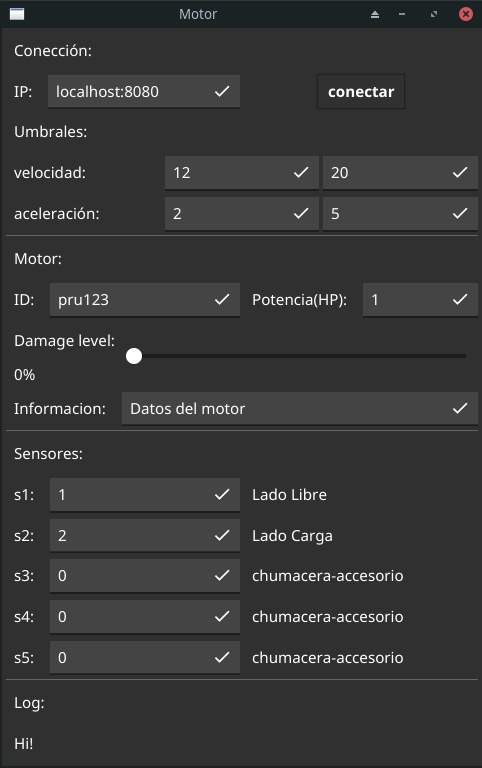
\includegraphics[width=\linewidth]{clients/ClienteSensoricaSinConectar.png}
        Interfaz de usuario para la conexion del cliente de sensorica. \label{img:fyne}
	\end{figure}

\subsubsection{Cliente Web}

Este cliente es el mas conocido, ya que es el que permite que se muestre la
información en el navegador Web. Esta constituido por las vistas general,
específica y exhaustiva, cada una de ellas representa una pagina Web separada y
todas fueron construidas utilizando el Framework de JavaScript \textbf{React}
y con HTML específicamente un Template de Django y CSS para dar estructura
básica y estilo respectivamente.

Se optó por utilizar un
estilo multi páginas con renderizado de lado servidor (específicamente del
servidor Web) por la necesidad de los cálculos avanzados y gráficas que
se deben realizar, además de los llamados importantes e interconexiones con la
API del servidor de Go y de las BBDD. Esto difiere con el paradigma tradicional de
React (monopagina de renderizado en servidor) pero permite optimizar recursos y
facilita expansiones a futuro.

Su estructura viene dada por las 3 paginas o sub aplicaciones que permiten:

\begin{itemize}
    \item General: conocer el estado general de un grupo de motores, indicando
        en código de colores (verde, amarillo, rojo) el nivel de daño que posee
        un motor. Este nivel es determinado por las muestras mas actuales de
        la información del motor y unos valores parámetros proporcionados en
        conjunto con los datos de los cuales se elaboró el modelo estadístico.

        Cabe resaltar que estos valores son una extrapolación empírica de la
        vibración en una planta específica, es configurable y puede variar dadas
        las características propias de cada instalación. Esto es debido a que
        las bases utilizadas en la instalación, los soportes, entre otros factores
        \textbf{causados por ignorar las normas de instalación} afectan las medidas.

    \item Específica:  permite el estudio del estado de un motor específico,
        es enviado el parámetro que lo identifica en el Url, al servidor.
        Permite observar
        una gráfica histórica y una tabla exportable a excel de sus características y
        evolución en el tiempo, siempre y cuando se tenga medición de ese periodo
        en la base de datos, asimismo permite solicitar la vista exhaustiva del
        mismo motor si es requerido un nivel mayor de análisis.

    \item Exhaustiva: esta vista incluye todo lo anterior de la vista específica,
        con la diferencia de que permite regresar al menú general en vez de hacer
        una vista exhaustiva; además, realiza un análisis en frecuencia
        del estado a tiempo real del motor. Este análisis se puede realizar si
        se tiene acceso en tiempo real con el motor, es decir,
        el servidor de \textbf{sensorica} debe tener una conexión con un sensor que se
        encargue de monitorear el respectivo motor permitiéndole así solicitar
        la información necesaria para hacer el análisis.

        Cabe resaltar que esta acción es tratada como una vista aparte ya que
        tiene un peso computacional relativamente alto asociado y, por ende,
        además de consumir recursos tiene una duración de carga de algunos
        segundos que deteriora la experiencia de usuario, por esto
        obtiene solamente por una solicitud explicita.
\end{itemize}





    
\subsection{COMPROBACIÓN DE LOS RESULTADOS}

Como se ha mencionado anteriormente, el trabajo consta de una gran cantidad de
puntos que han sido trabajados de forma modular con la finalidad
de maximizar la escalabilidad y de facilitar al máximo posible el realizar pruebas
a los módulos y a los acoples realizados. La comprobación debe de
 tomar en consideración 2 factores, los resultados técnicos, es decir
funcionalidades de la aplicación las cuales, como se mencionó anteriormente, no se
automatizaron por factores tiempo y cantidad de pruebas y, los resultados finales,
es decir la capacidad de la herramienta de facilitar el trabajo, mediante
las páginas generales, específicas y exhaustivas.

\subsubsection{Comprobación de resultados a nivel técnico}

Las fallas internas de los servidores, o de procesos de comunicación
con la base de datos, conllevan a la finalización de la ejecución del proceso
(aplicación) correspondiente; esto se hace para poder reiniciar el sistema y
agregar el error o falla catastrófica a un archivo (log) que sirve para seguir el
comportamiento del servidor.

En el caso del servidor de sensorica, estos errores son manejados de forma manual
y se utiliza la característica de Go \textbf{``panic"} para detener la ejecución, mas
específicamente un paquete de la librería estándar \textbf{``log"} con la función
\textbf{``log.Faltalf"}.
Por otro lado, el Framework de Django se encarga de esto, si el error es manejable;
algún problema en una petición, o algo no catastrófico, arroja una excepción y un
error 500, fallo interno en el servidor, y finaliza la petición; en el caso de no
poder ser recuperado finaliza el proceso.

La finalización del servidor es una práctica relativamente común ya que permite
el reinicio del proceso, esto se hace mediante una configuración interna al
momento de hacer \textbf{deploy} en el servidor, como se observa en la figura
\ref{img:ProcesosLinux}
es la configuración recomendada por DigitalOcean para un reinicio
continuo, en caso de falla, a intervalos de 5 segundos.


	\begin{figure}[H]
		\centering
        \caption{Configuración de proceso en Linux para reinicio automático de procesos}
        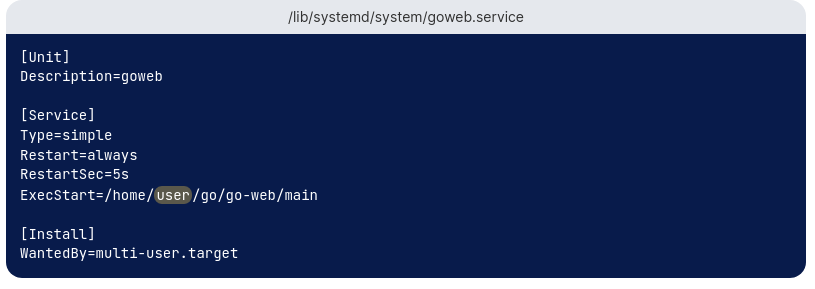
\includegraphics[width=\linewidth]{comprobacion_resultados/tecnicos/reinicio_servidor.png}

        \textcite{ConfiguracionProcesos}.
        \label{img:ProcesosLinux}
	\end{figure}

Por esta razón, las pruebas mas considerables son interconexiones y configuraciones
de seguridad y problemas de datos. es decir:

\begin{itemize}
    \item Prueba de no unicidad de la información, al haber múltiples
        clientes de sensorica enviando información sobre el mismo motor.

        Para esta posibilidad, se optó por una configuración que rechaza el
        segundo intento de conexión, es decir, se rechaza cualquier intento de
        conexión de motor con una conexión establecida previamente (que todavía
        exista), y su implementación se observa en la figura \ref{img:NoUnicidad}.
%
	\begin{figure}[H]
		\centering
        \caption{Prueba de error, no unicidad de información}
        \includegraphics[width=\linewidth]{comprobacion_resultados/tecnicos/NoUnicidadSensorica.png}

        logs: Izquierda cliente conectado, Centro cliente Rechazado, Derecha.
        Servidor.
        \label{img:NoUnicidad}
	\end{figure}
%
    \item Prueba de falla en la conexión de la base de datos.

        Cada servidor toma esta falla de una forma específica, en el caso del
        servidor de sensorica, esta es considerada una falla catastrófica, por
        lo que se finaliza la ejecución, como se observa en la figura
        \ref{img:NoBBDDSensorica}.

        Por otro lado, el servidor Web arroja una excepción, la cual es manejada
        internamente por Django y resuelta de forma que la petición es respondida
        con un error 500, falla interna del servidor, este error en la respuesta
        dada es manejado por el cliente y se observa en la figura
        \ref{img:NoBBDDWeb} .
%
    \begin{figure}[H]
		\centering
        \caption{Prueba de error, no BBDD Sensorica}
        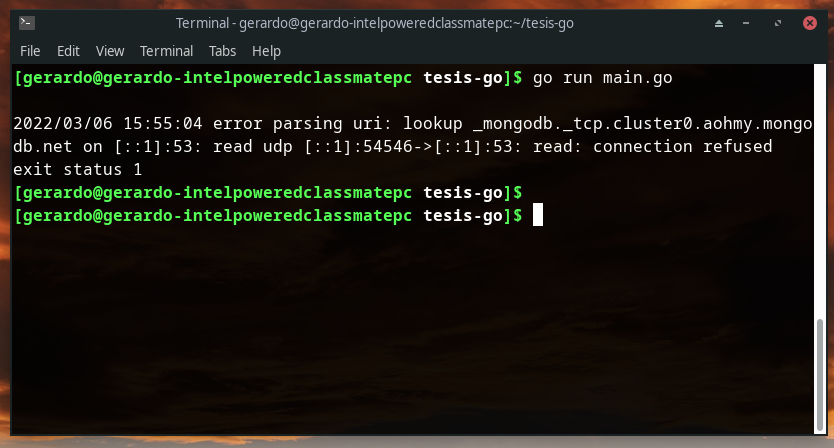
\includegraphics[width=\linewidth]{comprobacion_resultados/tecnicos/conexionInvalidaNoBBDDSensorica.png}

        El sistema no inicia por no poder conectarse a la BBDD.
        \label{img:NoBBDDSensorica}
	\end{figure}

    \begin{figure}[H]
		\centering
        \caption{Prueba de error, no BBDD Web}
        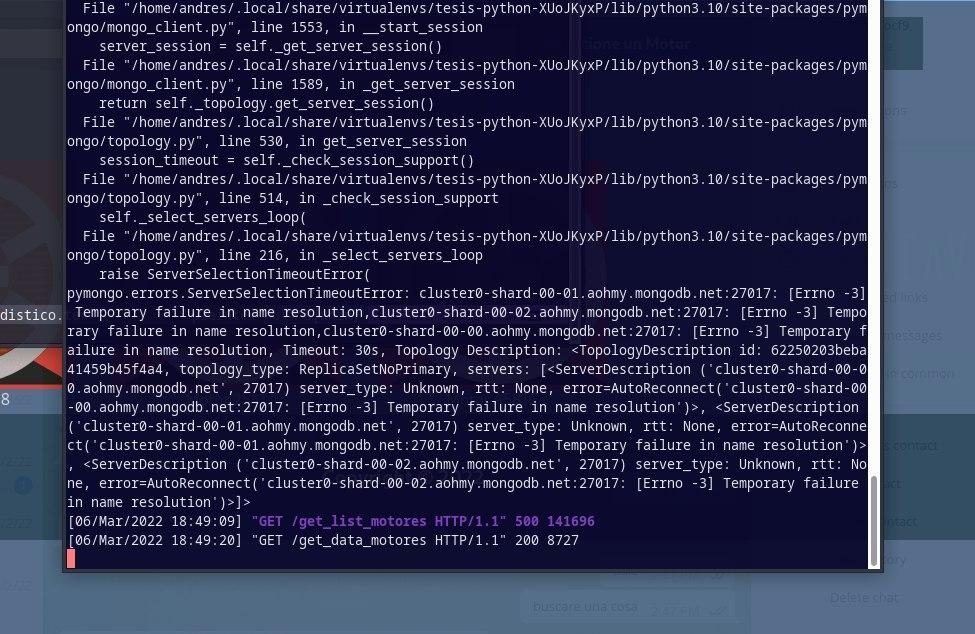
\includegraphics[width=\linewidth]{comprobacion_resultados/tecnicos/conexionInvalidaNoBBDDWeb.png}

        El sistema continua ejecución y resuelve el error con un error 500.
        \label{img:NoBBDDWeb}
	\end{figure}
%
    \item Prueba de solicitud de vista exhaustiva a un motor sin conexión
        establecida.

        Este caso corresponde al servidor de sensorica; al no haber una conexión
        con el sensor establecida no se pueden tomar las mediciones para una vista
        exhaustiva, estas deben ser en tiempo real, por lo tanto se responde
        con una error en la respuesta como se observa en la imagen \ref{img:ErrorExhaustiva}.
%

%
    \item Prueba de petición no completada en el cliente Web,
        información invalida (motor no existente) o error del servidor Web.

        En este caso se muestra al cliente un error por pantalla, como ventana
        emergente, y se redirige a la vista general como se observa en la
        figura \ref{img:SolicitudNoCompletada}.

    \begin{figure}[H]
		\centering
        \caption{Prueba de error, petición no completada en el cliente Web}
        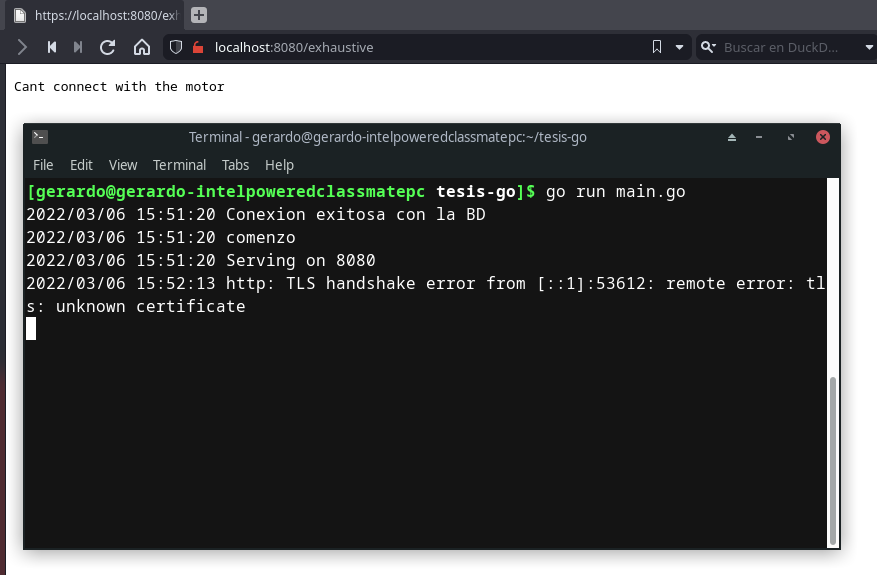
\includegraphics[width=\linewidth]{comprobacion_resultados/tecnicos/conexionInvalidaNoMotorSensorica.png}

        Solicitud  desde el navegador, para facilitar vista, al servidor
        sin motores conectados.
        \label{img:ErrorExhaustiva}
	\end{figure}

    \begin{figure}[H]
		\centering
        \caption{Prueba de error, petición exhaustiva inválida}
        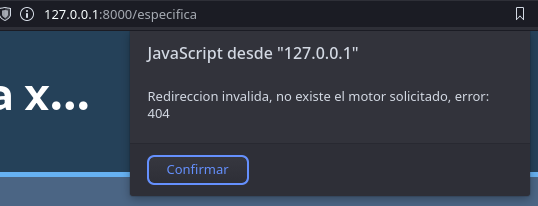
\includegraphics[width=\linewidth]{comprobacion_resultados/tecnicos/redireccionClienteWeb.png}

        Solicitud no completada en el cliente Web. \label{img:SolicitudNoCompletada}
	\end{figure}
\end{itemize}

\subsubsection{Comprobación de resultados finales}
Una vez terminado todo el proyecto se debieron rectificar que los requerimientos
solicitados, en terminos de parametros, sean cumplidos al igual que las graficas
resultantes, para las historicas como para el analisis en frecuencia, tengan
coherencia, dado esto se procedio de la siguiente forma:

\begin{itemize}
    \item Corroboración del análisis en nivel de daño básico (vista general)
        que se ajuste a los parámetros requeridos por el cliente.

        Para esta prueba se ingresaron 5 motores a la BBDD cuya informacion fue
        estrictamente configurada para cumplir los 3 estados de daño, y los
        2 valores frontera. Consiguiendo de esta forma cubrir todas las
        posibilidades, este resultado puede verse en la figura .

    \item Corroboración de las gráficas históricas.

        Esta verificaion es conseguida mediante la comparacion con los valores
        historicos, igual que para la prueba anterior, se ingreso un motor
        con valores de medicion faciles de seguir para corroborar la legibilidad
        y precision de la grafica, como se puede observar en la figura .

    \item Corroboración de la gráfica de la transformada de Fourier.

        En este caso se procedio a comparar la grafica obtenida mediante el
        algoritmo de python con una obtenida mediante el software Octave (version
        codigo abierta de Matlab), los resultados pueden verse en la figura .
\end{itemize}



    % UI, CLIENTE WEoB
    \begin{figure}[H]
        \centering
        \caption{Comprobación de los niveles en los motores}
        \begin{tabular}{m{6cm}m{6cm}}
            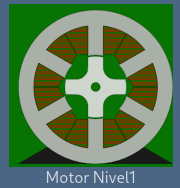
\includegraphics[width=6cm]{comprobacion_resultados/finales/n1.png}&
            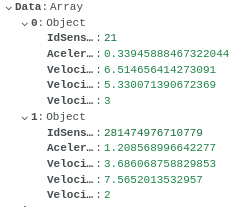
\includegraphics[width=6cm]{comprobacion_resultados/finales/n1mongo.png}\\
            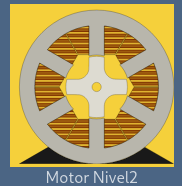
\includegraphics[width=6cm]{comprobacion_resultados/finales/n2.png}&
            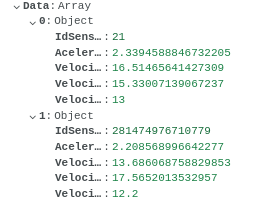
\includegraphics[width=6cm]{comprobacion_resultados/finales/n2mongo.png}\\
            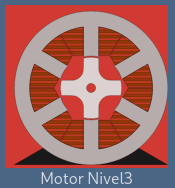
\includegraphics[width=6cm]{comprobacion_resultados/finales/n3.png}&
            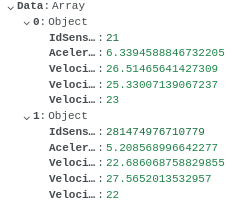
\includegraphics[width=6cm]{comprobacion_resultados/finales/n3mongo.png}
        \end{tabular}
        \label{img:NivelesMotores}
    \end{figure}

    \begin{figure}[H]
        \centering
        \caption{Comprobación de las fronteras en los motores}
        \begin{tabular}{m{6cm}m{6cm}}
            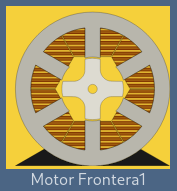
\includegraphics[width=6cm]{comprobacion_resultados/finales/f1.png}&
            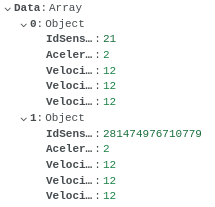
\includegraphics[width=6cm]{comprobacion_resultados/finales/f1mongo.png}\\
            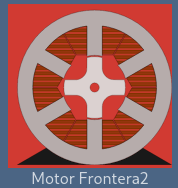
\includegraphics[width=6cm]{comprobacion_resultados/finales/f2.png}&
            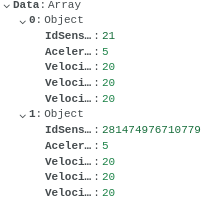
\includegraphics[width=6cm]{comprobacion_resultados/finales/f2mongo.png}
        \end{tabular}
        \label{img:FronterasEnLosMotores}
    \end{figure}

    \begin{figure}[H]
        \centering
        \caption{Comprobación gráficas históricas}
        \begin{tabular}{m{8cm}m{8cm}}
            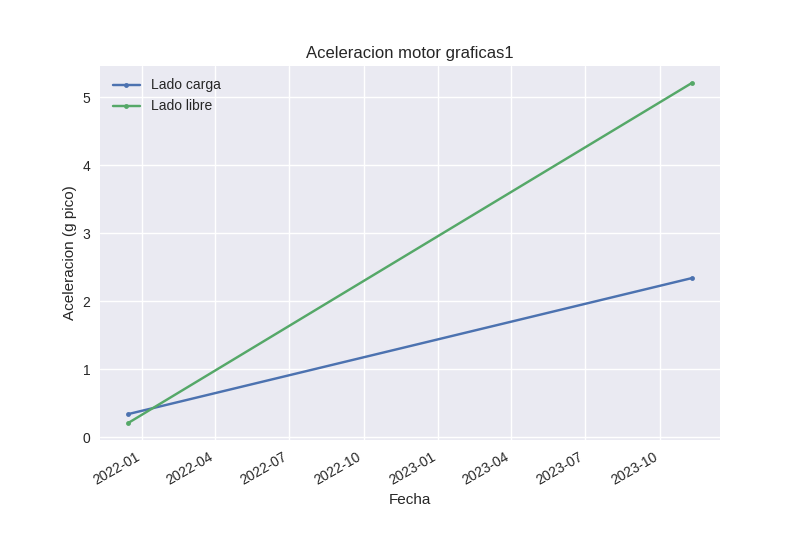
\includegraphics[width=8cm]{comprobacion_resultados/finales/as_graficas1.png}&
            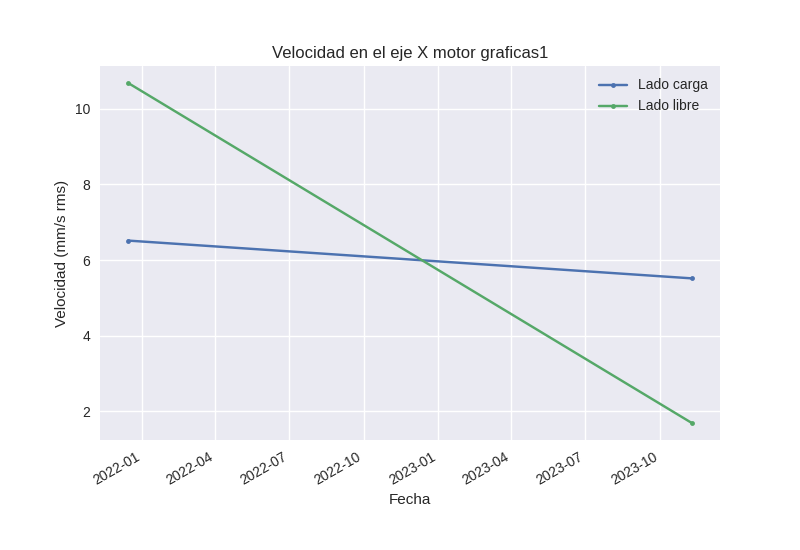
\includegraphics[width=8cm]{comprobacion_resultados/finales/vxs_graficas1.png}\\
            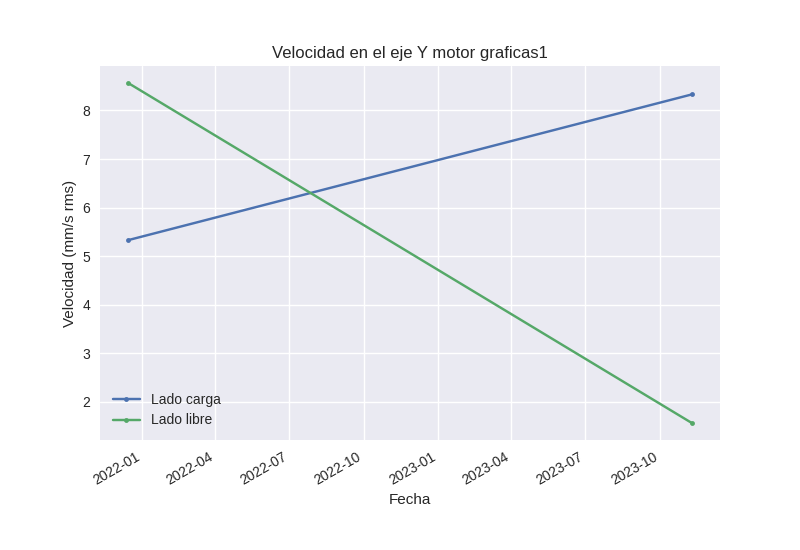
\includegraphics[width=8cm]{comprobacion_resultados/finales/vys_graficas1.png}&
            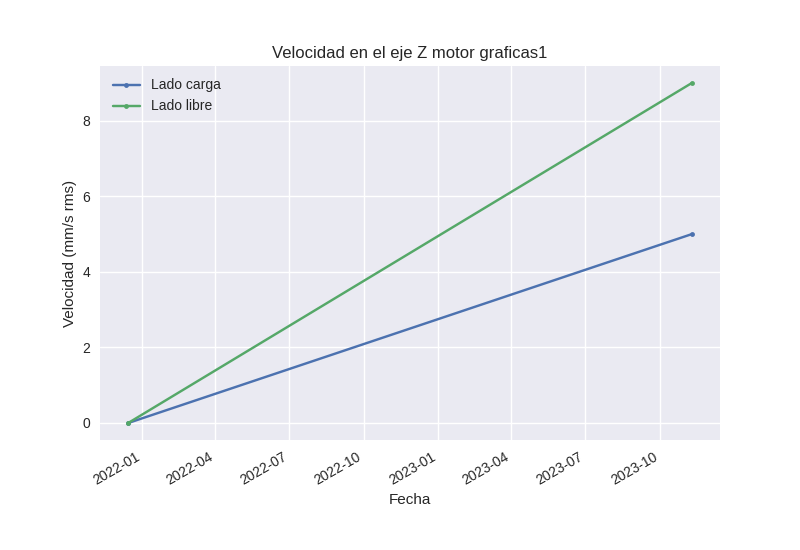
\includegraphics[width=8cm]{comprobacion_resultados/finales/vzs_graficas1.png}\\
            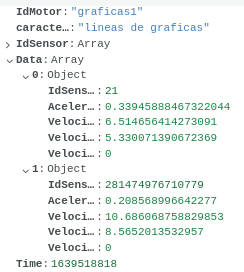
\includegraphics[width=8cm]{comprobacion_resultados/finales/graficas1Mongo1.png}&
            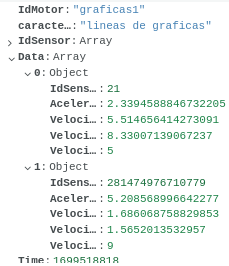
\includegraphics[width=8cm]{comprobacion_resultados/finales/graficas1Mongo2.png}\\
            \multicolumn{2}{c}{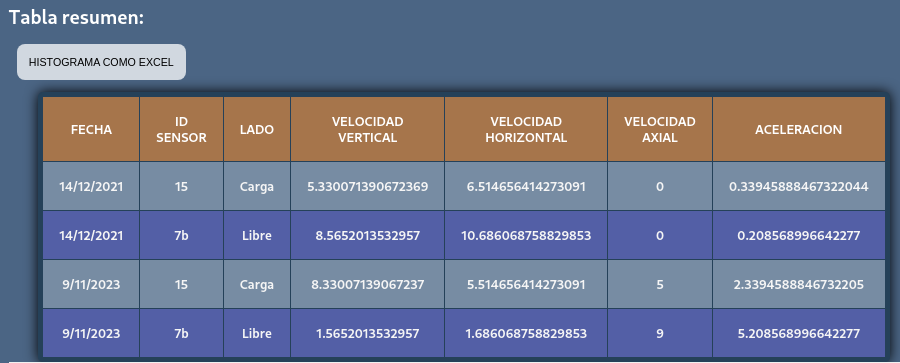
\includegraphics[width=12cm]{comprobacion_resultados/finales/tablaGraficas1.png}}
        \end{tabular}
        \label{img:GraficasHistoricas}
    \end{figure}

 %   \begin{figure}[H]
 %       \centering
 %       \caption{Comparación FFT python y octave}
 %       \begin{tabular}{m{16cm}}
 %           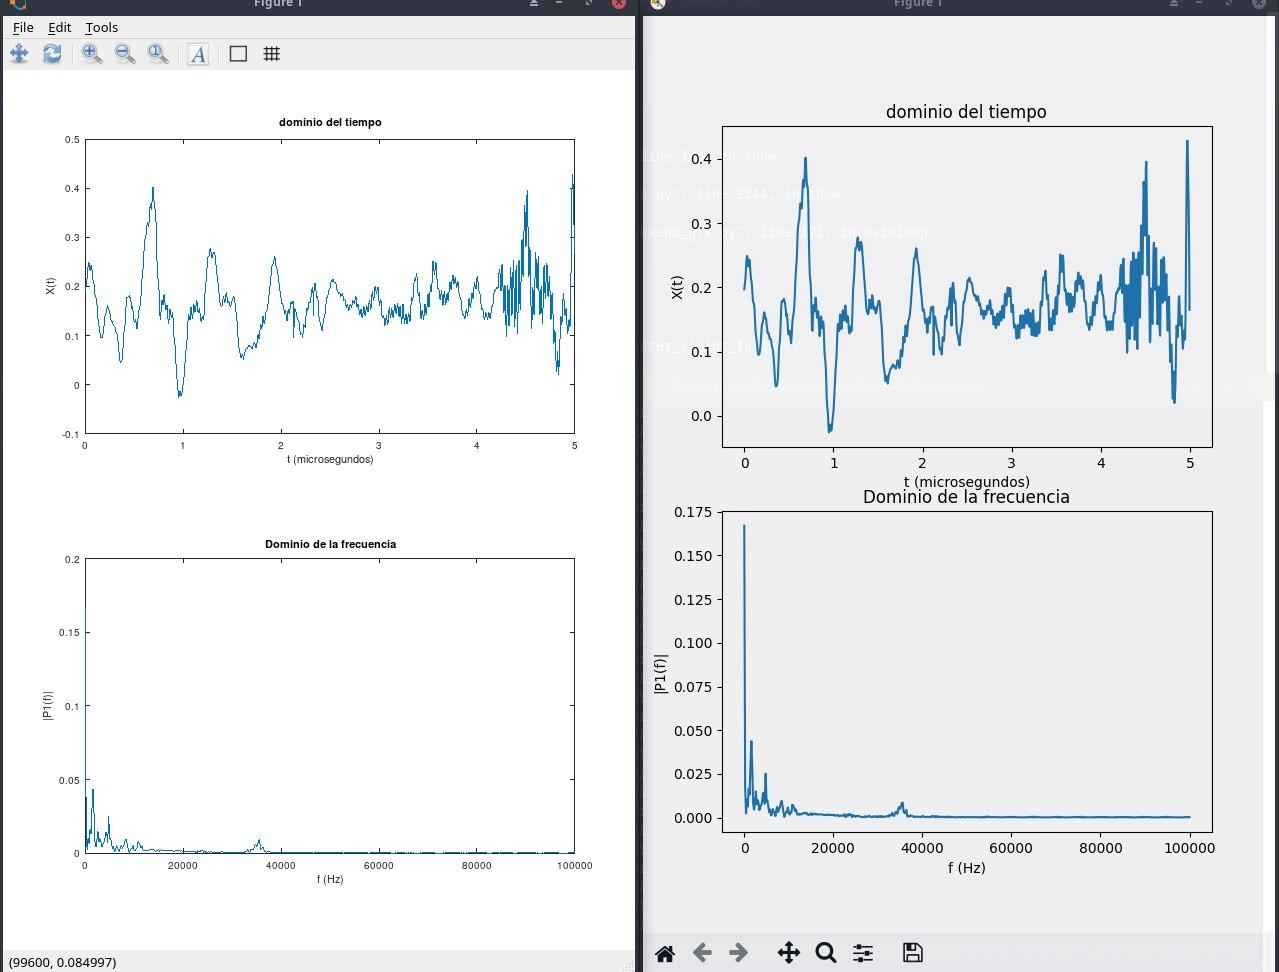
\includegraphics[width=16cm]{comprobacion_resultados/finales/comFFT1.png}\\
 %           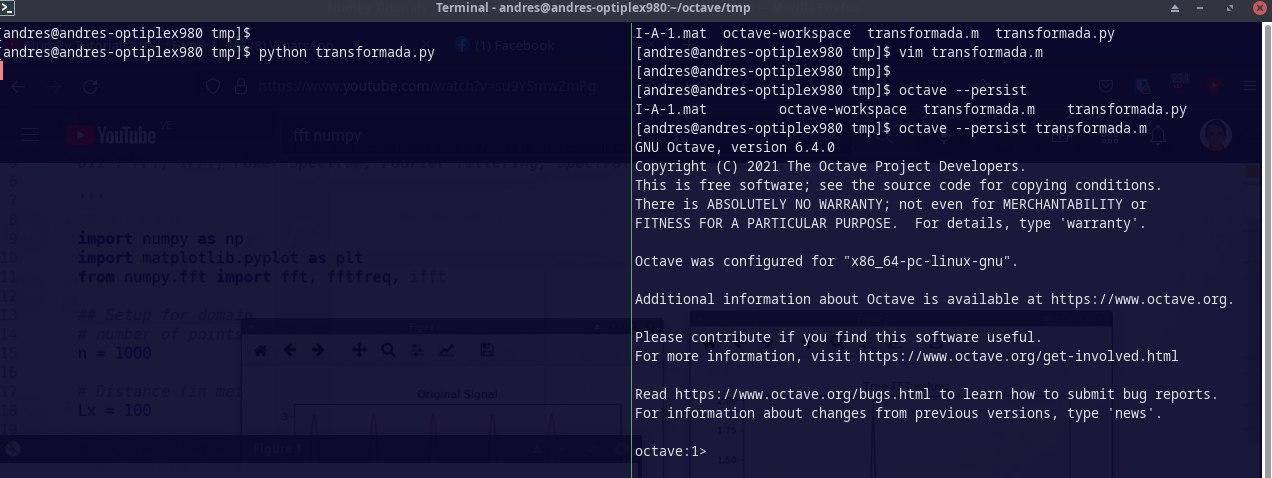
\includegraphics[width=16cm]{comprobacion_resultados/finales/comFFT1Terminales.png}
 %       \end{tabular}
 %       \label{img:FFTMidley}
 %   \end{figure}

    \begin{figure}[H]
        \centering
        \caption{FFT Octave vs Python datos del modelo}
            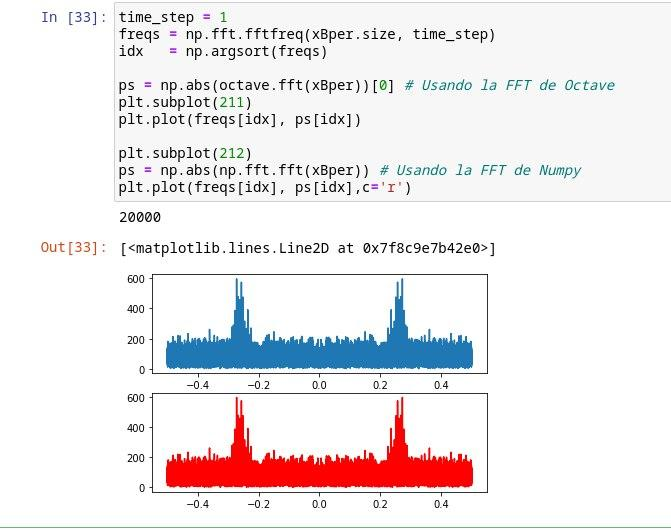
\includegraphics[width=16cm]{comprobacion_resultados/finales/comFFT2.png}
        \label{img:FFTSensores}
    \end{figure}
    \endgroup


%***************************************************
%**********  Capitulo 5  ***************************
%***************************************************
    \thispagestyle{empty}

\section{CONCLUSIONES Y RECOMENDACIONES}
\subsection{Conclusiones}
Tras la exposición de los resultados plasmados en el Capítulo IV, se pueden
plantear las siguientes conclusiones:

\begin{itemize}
    \item La investigación realizada ha sido de tipo aplicada y su naturaleza
        la clasifica como proyecto especial. Ésta ha consisitido en la creación
        de una herramienta computacional para el análisis de la vibracion en motores
        eléctricos mediante la implementación de dos servidores, uno de estilo
        microservicio, y un cliente Web, la cual puede ser alimentada mediante
        simulaciones, como es el caso del modelo estadistico y el sistema de
        sensorica, o mediante mediciones a tiempo real de cualquier sistema
        que respete las estructuras de datos empleadas.
        %
    \item Se deciden implementar multiples servicios, cada uno escrito con un
        lenguaje de programacion que satisface los requerimientos de velocidad,
        paralelismo y robustez necesarios para satisfacer los requerimientos de
        uso, ademas de una facil adecuacion y modificacion a las necesidades,
        de multiples clientes.
        %
    \item Existe una gran cantidad de lenguajes de programacion en la actualidad
        diseñados para satisfacer una gran cantidad de tareas en multiples campos,
        siendo Go y Python herramientas de gran poder y facil implementacion
        al momento de realizar servidores y API, ademas de la creacion de scripts
        para la automatizacion de procesos; de igual forma Python es increiblemente
        polifacetico y cuenta con una gran cantidad de librerias y Frameworks
        especialmente en el area de la ciencia de datos y estadistica; sin embargo
        en terminos de programacion Web a nivel cliente, es casi la unica
        posibilidad el utilizar HTML, CSS, JavaScript, presentando el ultimo la
        mayor variedad de Frameworks para agilizar el trabajo, siendo React uno
        de los mas grandes en la industria.
        %
    \item Se escoge implementar dos modelos estadisticos, uno para entregar el
        equivalente a mediciones diarias y otro para mediciones continuas a tiempo
        real necesarias para hacer un analisis en frecuencia; de esta forma se
        utilizaron distribuciones de probabilidad para representar 3 variables de interes,
        velocidad vertical, horizontal y aceleracion, expresadas de forma independiente
        como magnitud y angulo de la velocidad y aceleracion con las dos primeras
        siendo la representacion en coordenadas polares; las distribuciones que
        satisfacen de mejor manera estas variables fueron la distribucion Burr
        de tipo III para la magnitud de velocidad y aceleración, y la distribucion
        normal para el angulo. De esta forma, se obtienen las mediciones diarias
        y con un modelo de señal no estadistico ajustado a la amplitud dada por
        el modelo de la aceleración y una gaussiana para simular ruido, se obtienen
        las mediciones continuas.
        %
    \item Para facilitar la accesibilidad al modelo se implementó una API Web con
        el framework FastAPI y dos endpoints que entregan la información especificada
        en el Url via parametros de configuracion, nivel de daño (un numero del 0 al 10)
        y el identificador unico del motor que tiene asociado.
        %
    \item Una vez obtenidas las salidas del podelo estadistico, se procede con
        la implementación del analisis en frecuencia, esto se logra mediante una
        transformada rapida de Fourier (FFT) lo que permite llevar la señal
        discretizada (mediciones a tiempo real) al dominio de la frecuencia
        y posteriormente graficarla; todo esto se logra mediante las librerias
        \textbf{numpy} y \textbf{matplotlib} de Python.
        %
    \item  Se utilizo una base de datos no relacional, \textbf{MongoDB}, en forma
        de microservicio con la empresa \textbf{MongoDB Atlas} la cual permite
        la creacion de un \textbf{cluster} gratuito para finalidades de practicas
        y estudios, capaz de almacenar una cierta cantidad de información e
        implementar diversas bases de datos y colecciones para las mismas, siempre
        que no se exceda este limite; esta base de datos llamada \textbf{tesis}
        contiene 2 colecciones, una se encarga de almacenar la informacion de las
        mediciones diarias y la otra de almacenar los identificadores unicos que
        representan a los motor de los que se posee informacion.
        %
    \item La automatización de procesos es fundamental para agilizar las tareas y
        la forma mas sencilla y optima de hacerlo es mediante un script; para
        llenar la base de datos se utilizo uno escrito en Go el cual acepta
        configuracion al momento de la ejecucion via parametros, siendo obligatorios
        la especificación de los identificadores unicos correspondientes al motor
        y los primeros 2 sensores.
        %
    \item Se crearon 2 microservicios como servidores, el primero llamado
        \textbf{servidor de sensorica}
        se encarga de la comunicacion con los sensores, simulados mediante el
        \textbf{cliente de sensorica} y el \textbf{modelo estadistico}, y la
        entrega de la informacion tomada a tiempo real necesaria para el analisis
        en frecuenca. Por otro lado, el otro microservicio, \textbf{servidor Web},
        se encarga de satisfacer las peticiones Web al enviar el HTML-CSS-JavaScript
        necesario para mostrar la pagina, ademas de los archivos estaticos e
        informacion requeridos por los mismos para mostrar el estado de los motores
        dependiendo del nivel de analisis solicitado.
        %
    \item Para facilitar la utilizacion del modelo estadistico y la conexion con
        el microservicio de \textbf{sensorica} se implemento un \textbf{cliente de
        sensorica} escrito en Go el cual permite especificar las caracteristicas
        inherentes al motor (Identificador del motor y de los sensores, caracteristicas, etc)
        y al daño existente en el mismo (en una escala del 1 al 10), ademas permite
        especificar la direccion IP, o puerto local, al cual se conectara.
        %
    \item Se crearon 3 vistas para el cliente Web, estas son:
        \begin{enumerate}
            \item \textbf{General},
                tiene el menor grado de estudio ya que permite conocer el estado de todos
                los motores registrados en la BBDD, esto se consigue mediante paginacion
                en una ventana, esta muestra 12 motores por vez y permite mover el indice
                para mostrar los siguientes 12, regresarse e ir automaticamente al inicio,
                ademas existe una ventana de busqueda que permite especificar el identificador
                unico del motor del cual se quiere obtener la informacion.
                %
            \item \textbf{específica}, tiene un grado de estudio intermedio dado que
                permite conocer la evolucion historica del motor mediante graficas
                y una tabla exportable a Excel; adicionalmente permite solicitar
                la vista exhaustiva.
                %
            \item \textbf{exhaustiva}, tiene el mayor grado de estudio ya que
                solicita mediciones a tiempo real de la aceleración del motor
                y las descompone en frecuencia, permitiendo observar una grafica
                de las frecuencias y magnitudes de las mismas en las que vibra
                el motor; adicionalmente muestra toda la informacion de la
                vista específica.
        \end{enumerate}
        %
    \item Dado el tiempo de desarrollo y la complejidad del sistema no se
        pueden escribir \textbf{test} automatizados, sin embargo es absolutamente
        necesario el realizar pruebas a un software para garantizar su funcionamiento,
        por esta razon se probó manuealmente el sistema en los puntos claves
        e interconexiones, es decir, se comprobó:
        \begin{enumerate}
            \item La unicidad de la información.
            \item Fallas de conexion con el microservicio de base de datos.
            \item Solicitud de información a tiempo real a un motor sin conexión
                establecida.
            \item Peticiones invalidas en el servidor Web
        \end{enumerate}
        %
    \item Una vez establecido el sistema, se procedio a comprobar que cumpliera
        los requerimientos minimos solicitados por el cliente, es decir, se
        verificaron la clasificación en los distintos niveles de daño de acuerdo
        a las especificaciones del cliente, se corroboró la coherencia y legibilidad
        de las graficas historicas y de la grafica del analisis en frecuencia.
        %
\end{itemize}



\subsection{Recomendaciones}
\begin{itemize}
    \item Debido al costo que implica no se realizaron placas de adquisición de
        datos y tampoco se obtuvo data en tiempo real de motores eléctricos
        para la elaboración de este trabajo, pero el mismo puede ser
        complementado implementando dichos dispositivos.

    \item Para su uso empresarial la aplicación requiere de un sistema de
        autentificación y de seguridad para que solo los usuarios con los
        privilegios correctos puedan acceder a la información, esto
        probablemente requiera el uso de otra base de datos preferiblemente una
        base de datos relacional.

    \item Un sistema de notificaciones configurable por el usuario, para
        observar si algún motor recibe una medida fuera de los valores normales
        puede ser una gran ayuda al operador de la aplicación en el diagnóstico
        de fallas de forma temprana.

    \item Debido a la complejidad de las conexiones HTTP2 una alternativa es el
        uso de Websockets los cuales permiten una conexión bidireccional sin la
        complejidad del nuevo protocolo pero posee su propia serie de
        desventajas las cuales tienen que ser evaluadas con los requerimientos
        de la aplicación. Otra alternativa aún no disponible pero en un futuro
        cercano posiblemente lo este, es HTTP3 la cual está siendo discutida
        por el comité del estándar HTTP para corregir las fallas de la última
        versión.

    \item Las pruebas fueron realizadas de forma manual pero una decisión que
        puede minimizar el tiempo de depuración y evitar las fallas en
        producción es el uso de pruebas automatizadas pero eso implica un coste
        en el tiempo de desarrollo dedicado al diseño de las pruebas por lo
        tanto la elección de usarlas o no dependerá de la experiencia previa
        del programador con este tipo de metodología de desarrollo.

    \item El ecosistema de librerías y frameworks frontend es muy cambiante por
        lo tanto la elección de las herramientas debe ser realizada de acuerdo
        a las tecnologías más populares al momento del desarrollo.

    \item  Si bien no se llegó a utilizar Julia sigue siendo un lenguaje con
        mucho potencial tratando de incorporar ventajas de lenguajes
        interpretados como python y lenguajes compilados como Fortran. Su
        principal desventaja es lo joven que es pero a futuro puede llegar ser
        uno de los lenguajes más dominantes en el campo científico.

\end{itemize}

    %Conclusiones y Recomendaciones (que concluyo del trabajo)
    %que informacion se obtuvo de cada especifico,
    %que cosas de informacion adicional se nos dio mientras
    %desarrollamos

    % 1min aprox dedicado a cada lamina
    % No necesariamente debe de seguirse el orden del trabajo

\end{refsegment}

\begingroup
    \spacing{1.2}
    \setlength\bibitemsep{1.8\itemsep}

	\newpage
	\printbibliography[segment=1,title={\centering{REFERENCIAS BIBLIOGRÁFICAS}}]
    \nocite{*}
    \printbibliography[notkeyword={b1},title={\centering{BIBLIOGRAFÍA}}]
\endgroup
%***************************************************
%**********  Anexos      ***************************
%***************************************************

\titleformat{\section}[display]
%{\normalfont\bfseries\LARGE}{}{3pt}{ANEXO \thesection. \filcenter \LARGE}
{\normalfont\bfseries\LARGE}{ANEXO \thesection}{3pt}{\filcenter \LARGE}

\appendix
\spacing{1.5}
\counterwithin{figure}{section}


\thispagestyle{empty}
\addcontentsline{toc}{section}{ANEXOS}
%\setcounter{figure}{0}
\phantom{}
\vfill
\begin{center}
{\Huge ANEXOS}
\end{center}
\vfill
\phantom{}

    \subsection{ANEXO A. Manual de Uso e Instalación}

La herramienta computacional para el análisis de vibración en motores eléctricos
facilita el conocimiento del estado actual de los motores en una planta al mismo
tiempo que permite realizar estudios de evolución históricos y de vibración en
frecuencia, permitiendo de este modo conocer en profundidad que motores podrían
fallar y cual será el elemento, mecánico, que lo hará. Esto permite la realización
de un mantenimiento predictivo, facilitando y mejorando la efectividad y
coordinación de las paradas programadas en una empresa.

Esta herramienta es un sistema Web por lo cual \textbf{NO REQUIERE INSTALACIÓN
EN LA COMPUTADORA}, solo se debe acceder al sitio Web (servidor) el cual se
utilice como \textbf{HOST} para esta.

Para facilitar el acceso al usuario, esta consta de 3 paginas principales,
general, especifica y exhaustiva, además consta de 2 elementos fijos que son el
\textbf{Header}, mostrando la información de la planta y además permitiendo
el regreso a la vista principal (general),  solicitar ayuda y muestra en que
vista se encuentra en el momento. Esto se puede observar en la figura
\ref{img:HeaderHerramienta}.

    \begin{figure}[H]
		\centering
        \caption{Header de la herramienta computacional. }
        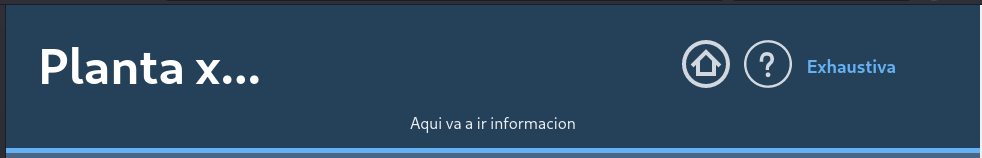
\includegraphics[width=\linewidth]{ManualUsuario/header.png}
        \label{img:HeaderHerramienta}
	\end{figure}

La otra vista constante es la del \textbf{Footer} que ofrece los derechos de autor
y copyright.

    \begin{figure}[H]
		\centering
        \caption{Footer de la herramienta computacional. }
        
\includegraphics[width=\linewidth]{ManualUsuario/footer.png}
        \label{img:FooterHerramienta}
	\end{figure}

El resto de la pantalla se modifica de acuerdo a que pestaña (vista) se observa,
esto es:

\subsubsection{Vista General}
Es la vista principal de la aplicación, esta diseñada para un monitoreo constante
lo que implica que recarga la información cada cierto tiempo (por defecto 30s)
este periodo puede ser modificado únicamente por código y si se desea cambiar debe
comunicarse con el proveedor de servicio.

Esta ventana, se observa en la figura \ref{img:vistaGeneralManual}
cuenta de dos partes fundamentales:

    \begin{figure}[H]
		\centering
        \caption{Vista de la pestaña general de la herramienta computacional. }
        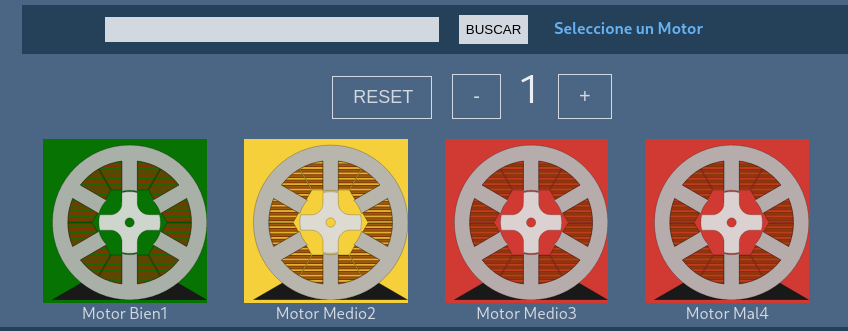
\includegraphics[width=\linewidth]{ManualUsuario/general.png}
        \label{img:vistaGeneralManual}
	\end{figure}

La primera es el despliegue de motores
con un máximo de 12 motores por "pagina" (para modificar esta cantidad comunicarse
con el proveedor de servicios) los cuales indican su código o identificador en
su parte inferior (este código se ingresa al registrar el motor, se recomienda sea
el mismo del de mantenimiento para facilitar su utilización) y un diagrama de
motor con un fondo de color con código correspondiente a su estado, nivel de
vibración y aceleración ajustado a los parámetros solicitados (modificaciones con
el proveedor del servicio); este código es :

\begin{itemize}
    \item  verde: bien.
    \item amarillo: primera alerta.
    \item rojo: segunda alerta.
\end{itemize}

la segunda parte de interés es el buscador y control de paginación, se observa en
la figura \ref{img:buscadoreGeneral}, el buscador permite solicitar la vista
especifica de cualquier motor, buscando por el Identificador del mismo;
el control de paginación permite mostrar otros motores al "pasar" la pagina,
de igual forma permite regresar directamente al principio con el botón de
\textbf{RESET}.

    \begin{figure}[H]
		\centering
        \caption{Controles de paginación en la vista principal. }
        
\includegraphics[width=\linewidth]{ManualUsuario/controles.png}
        \label{img:buscadoreGeneral}
	\end{figure}


\subsubsection{Vista Especifica}
Esta vista permite un nivel de estudio superior ya que es solamente enfocada
a un motor y ofrece la información histórica del mismo, esto lo hace mediante
gráficas y una tabla exportable a Excel.

tiene 3 secciones de trascendencia:

la primera es un encabezado resumen,
se puede apreciar en \ref{img:especificaHeaderManual}; en este se encuentra
el estado del motor como en la vista general, un enlace para solicitar la
vista Exhaustiva y un mensaje con las características del motor o
comentarios adicionales añadidos al momento de la incorporación del motor al
sistema.

    \begin{figure}[H]
		\centering
        \caption{Sección de mensaje en la vista especifica. }
        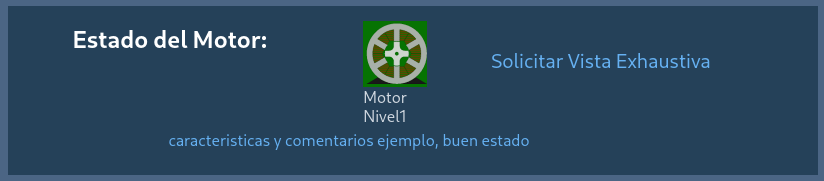
\includegraphics[width=\linewidth]{ManualUsuario/especificaMensaje.png}
        \label{img:especificaHeaderManual}
	\end{figure}

La segunda es una serie de gráficas de toda la información histórica, separada
por ejes (x,y,z) y de la aceleración, se muestran después de la palabra
\textbf{Histogramas}, como se observa en la figura \ref{img:especificaGraficasManual}.

    \begin{figure}[H]
		\centering
        \caption{Sección de gráficas en la vista especifica. }
        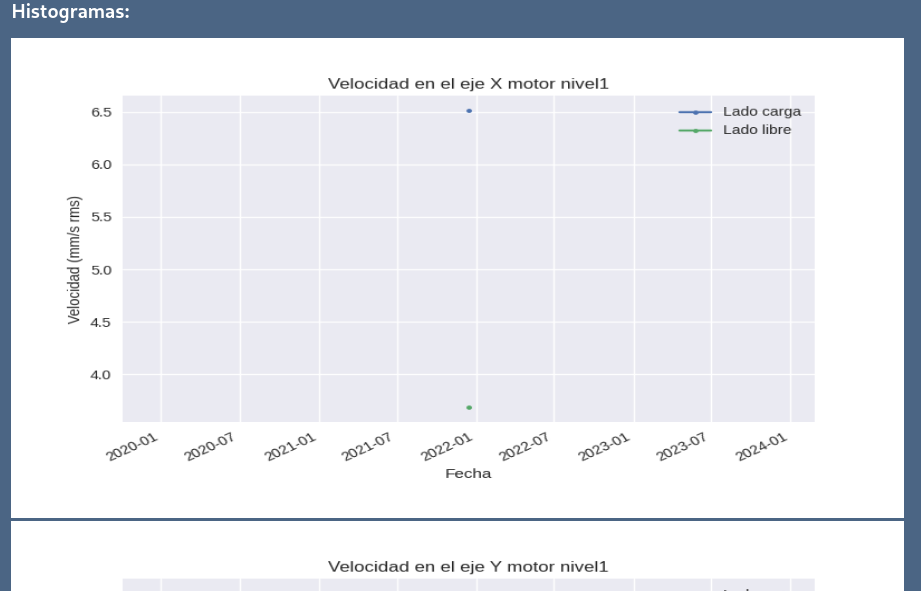
\includegraphics[width=\linewidth]{ManualUsuario/especificaGraficas.png}
        \label{img:especificaGraficasManual}
	\end{figure}

La tercera es una tabla, como se observa en \ref{img:especificaTablaManual}
exportable a Excel, mediante el botón, con toda la información de las mediciones
a lo largo de la historia del sistema, esta posee los campos de:
\begin{itemize}
    \item fecha, en la cual se tomo la medición.
    \item Id Sensor, identificador único, numero de serial, que posee el sensor
        (hardware), asociado.
    \item Lado, ubicación en la cual se tomo la medición, lado libre, lado con
        carga o chumaceras y acoples.
    \item Velocidad vertical, medición de la velocidad, en mm/s, medición rms
    \item Velocidad Horizontal, medición de la velocidad, en mm/s, medición rms
    \item Velocidad Axial, medición de la velocidad, en mm/s, medición rms
    \item Aceleración, medición de la aceleración, en \textbf{g} .
\end{itemize}

\textbf{Nota,} si la tabla no posee todos los campos en su navegador, selecciónela
y utilice las flechas del teclado para redirigirla, o reduzca el tamaño de su
pantalla.

    \begin{figure}[H]
		\centering
        \caption{Sección de la tabla en la vista especifica. }
        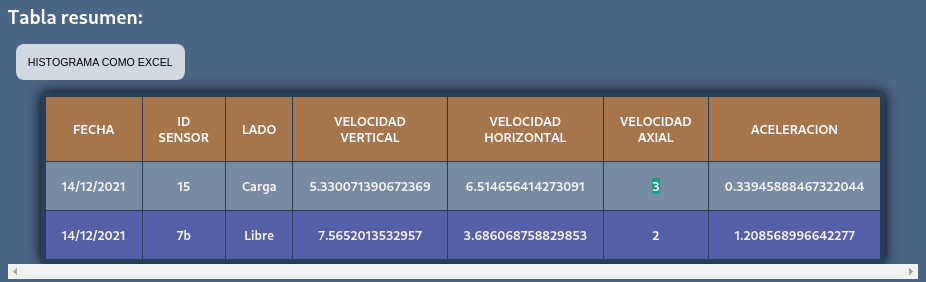
\includegraphics[width=\linewidth]{ManualUsuario/especificaTabla.png}
        \label{img:especificaTablaManual}
	\end{figure}


\subsubsection{Vista Exhaustiva}
Esta vista incluye las mismas características de la vista especifica pero sufre
una modificación en el encabezado resumen, como se puede apreciar en la figura
\ref{img:exhaustivaMensajeManual}
este redirige a la vista principal.

    \begin{figure}[H]
		\centering
        \caption{Sección de mensaje en la vista exhaustiva. }
        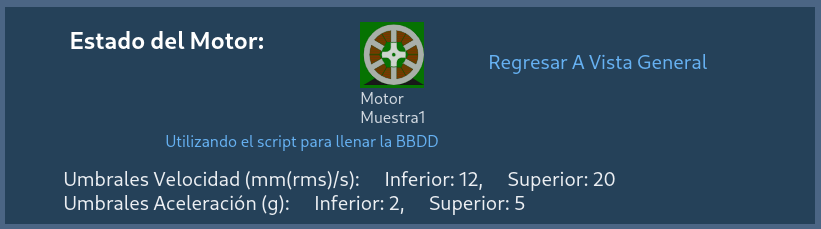
\includegraphics[width=\linewidth]{ManualUsuario/exhaustivaMensaje.png}
        \label{img:exhaustivaMensajeManual}
	\end{figure}



La otra modificación es que se añade otra sección de gráfica en la cual se muestra
la salida de un estudio en frecuencia, permitiendo este su análisis; se observa en
la figura \ref{img:exhaustivaGraficaFourierManual}


    \begin{figure}[H]
		\centering
        \caption{Sección de gráfica de frecuencia en la vista exhaustiva. }
        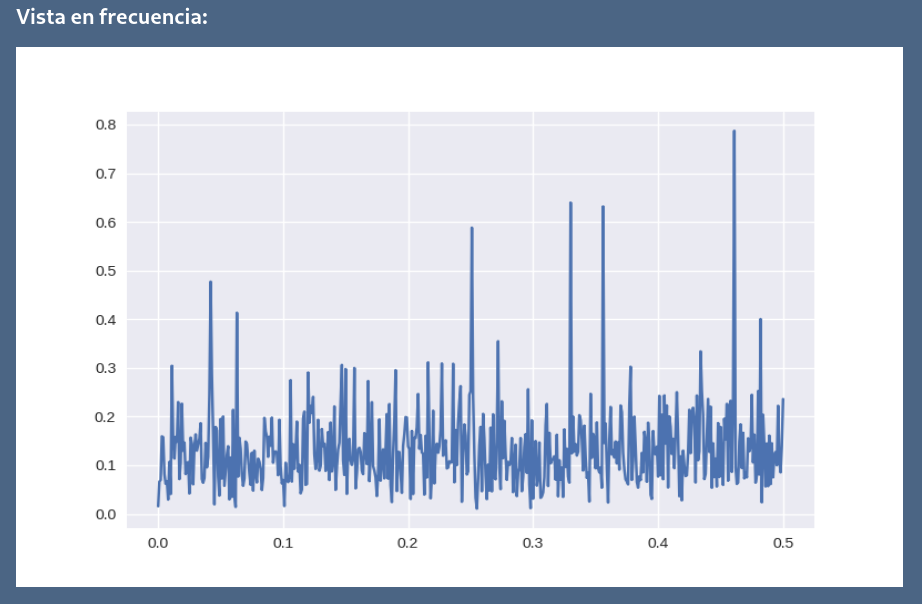
\includegraphics[width=\linewidth]{ManualUsuario/exhaustivaGraficaFourier.png}
        \label{img:exhaustivaGraficaFourierManual}
	\end{figure}






\end{document}
